%%%%%%%%%%%%%%%%%%%%%%%%%%%%%%%%%%%%%%%%%%%%%%%%%%%%%%%%%%%%%%%
%% OXFORD THESIS TEMPLATE

% Use this template to produce a standard thesis that meets the Oxford University requirements for DPhil submission
%
% Originally by Keith A. Gillow (gillow@maths.ox.ac.uk), 1997
% Modified by Sam Evans (sam@samuelevansresearch.org), 2007
% Modified by John McManigle (john@oxfordechoes.com), 2015
% Modified by Ulrik Lyngs (ulrik.lyngs@cs.ox.ac.uk), 2018, for use with R Markdown
%
% Ulrik Lyngs, 25 Nov 2018: Following John McManigle, broad permissions are granted to use, modify, and distribute this software
% as specified in the MIT License included in this distribution's LICENSE file.
%
% John tried to comment this file extensively, so read through it to see how to use the various options.  Remember
% that in LaTeX, any line starting with a % is NOT executed.  Several places below, you have a choice of which line to use
% out of multiple options (eg draft vs final, for PDF vs for binding, etc.)  When you pick one, add a % to the beginning of
% the lines you don't want.


%%%%% CHOOSE PAGE LAYOUT
% The most common choices should be below.  You can also do other things, like replacing "a4paper" with "letterpaper", etc.

% This one will format for two-sided binding (ie left and right pages have mirror margins; blank pages inserted where needed):
%\documentclass[a4paper,twoside]{templates/ociamthesis}
% This one will format for one-sided binding (ie left margin > right margin; no extra blank pages):
%\documentclass[a4paper]{ociamthesis}
% This one will format for PDF output (ie equal margins, no extra blank pages):
%\documentclass[a4paper,nobind]{templates/ociamthesis}
%UL 2 Dec 2018: pass this in from YAML
\documentclass[a4paper, nobind]{templates/ociamthesis}
\usepackage{mathptmx}

% UL 30 Nov 2018 pandoc puts lists in 'tightlist' command when no space between bullet points in Rmd file
\providecommand{\tightlist}{%
  \setlength{\itemsep}{0pt}\setlength{\parskip}{0pt}}
 
% UL 1 Dec 2018, fix to include code in shaded environments

%UL 2 Dec 2018 reduce whitespace around verbatim environments
\usepackage{etoolbox}
\makeatletter
\preto{\@verbatim}{\topsep=0pt \partopsep=0pt }
\makeatother

%UL 26 Mar 2019, enable strikethrough
\usepackage[normalem]{ulem}

%UL 15 Oct 2019, enable link highlighting to be turned off from YAML
\definecolor{darkblue}{rgb}{0, 0, 0.5}
\usepackage[pdfpagelabels,
    colorlinks=true,
    citecolor=darkblue,
    filecolor=darkblue,
    urlcolor=darkblue,
    hidelinks=]{hyperref}
\hypersetup{
    colorlinks=true,
    citecolor=darkblue,
    filecolor=darkblue,
    urlcolor=darkblue,
    linkcolor=black,
}

%%%%% SELECT YOUR DRAFT OPTIONS
% Three options going on here; use in any combination.  But remember to turn the first two off before
% generating a PDF to send to the printer!

% This adds a "DRAFT" footer to every normal page.  (The first page of each chapter is not a "normal" page.)

% This highlights (in blue) corrections marked with (for words) \mccorrect{blah} or (for whole
% paragraphs) \begin{mccorrection} . . . \end{mccorrection}.  This can be useful for sending a PDF of
% your corrected thesis to your examiners for review.  Turn it off, and the blue disappears.
\correctionstrue

%%%%% BIBLIOGRAPHY SETUP
% Note that your bibliography will require some tweaking depending on your department, preferred format, etc.
% The options included below are just very basic "sciencey" and "humanitiesey" options to get started.
% If you've not used LaTeX before, I recommend reading a little about biblatex/biber and getting started with it.
% If you're already a LaTeX pro and are used to natbib or something, modify as necessary.
% Either way, you'll have to choose and configure an appropriate bibliography format...

% The science-type option: numerical in-text citation with references in order of appearance.
% \usepackage[style=numeric-comp, sorting=none, backend=biber, doi=false, isbn=false]{biblatex}
% \newcommand*{\bibtitle}{References}

% The humanities-type option: author-year in-text citation with an alphabetical works cited.
% \usepackage[style=authoryear, sorting=nyt, backend=biber, maxcitenames=2, useprefix, doi=false, isbn=false]{biblatex}
% \newcommand*{\bibtitle}{Works Cited}

%UL 3 Dec 2018: set this from YAML in index.Rmd
\usepackage[style=authoryear, sorting=nyt, backend=biber, maxcitenames=1, mincitenames=1, maxbibnames=100, minbibnames=100, useprefix, doi=false, url=false, isbn=false, uniquename=false]{biblatex}
\newcommand*{\bibtitle}{\textbf{Bibliography}}

% Embed reference URL under the title inside bibliography
\newbibmacro{string+url}[1]{%
  \iffieldundef{url}{#1}{\href{\thefield{url}}{#1}}
}
\DeclareFieldFormat{title}{\usebibmacro{string+url}{\mkbibemph{#1}}}
\DeclareFieldFormat*{title}{\usebibmacro{string+url}{\mkbibquote{#1}}}

% Comma between author and year in citations
\renewcommand*{\nameyeardelim}{\addcomma\space}

% This makes the bibliography left-aligned (not 'justified') and slightly smaller font.
\renewcommand*{\bibfont}{\raggedright\small}

% Change this to the name of your .bib file (usually exported from a citation manager like Zotero or EndNote).
\addbibresource{references.bib}


% Uncomment this if you want equation numbers per section (2.3.12), instead of per chapter (2.18):
%\numberwithin{equation}{subsection}


%%%%% THESIS / TITLE PAGE INFORMATION
% Everybody needs to complete the following:
\title{Application of GLM Advancements\\
to Non-Life Insurance Pricing}
\author{Leonardo Stincone}
\universityname{Università degli Studi di Trieste}
\departmentname{Scienze Economiche, Aziendali, Matematiche e Statistiche}
\degreedef{Tesi di Laurea}
\degreename{Scienze Statistiche e Attuariali}
\degreeclass{LM-83}
\academicyear{2019 - 2020}
\degreedate{March 2021}
\advisorname{Prof.~Francesco Pauli}
%\coadvisorname{}
\degreedate{March 2021}

%%%%% YOUR OWN PERSONAL MACROS
% This is a good place to dump your own LaTeX macros as they come up.

% To make text superscripts shortcuts
	\renewcommand{\th}{\textsuperscript{th}} % ex: I won 4\th place
	\newcommand{\nd}{\textsuperscript{nd}}
	\renewcommand{\st}{\textsuperscript{st}}
	\newcommand{\rd}{\textsuperscript{rd}}


% For the Title Page with Italian style (frontespizio)
\usepackage[nouppercase]{frontespizio}

% For \cancel{} in equation
\usepackage[makeroom]{cancel}

% For bold symbol in equations
\usepackage{bm}

% For multiline cells in tables
\usepackage{makecell}

% % For Acronyms
% % % 
% \newacronym{glm}{GLM}{Generalized Linear Model}
% \newacronym{gam}{GAM}{Generalized Additive Model}

% For mathscr font in equations
\usepackage{mathrsfs}



%%%%%%%%%%%%%%%%%%%%%%%%%%%%%%%%%%%%%%%%%%%
%%%%% THE ACTUAL DOCUMENT STARTS HERE %%%%%
%%%%%%%%%%%%%%%%%%%%%%%%%%%%%%%%%%%%%%%%%%%
\usepackage{amsthm}
\newtheorem{theorem}{Theorem}[chapter]
\newtheorem{lemma}{Lemma}[chapter]
\newtheorem{corollary}{Corollary}[chapter]
\newtheorem{proposition}{Proposition}[chapter]
\newtheorem{conjecture}{Conjecture}[chapter]
\theoremstyle{definition}
\newtheorem{definition}{Definition}[chapter]
\theoremstyle{definition}
\newtheorem{example}{Example}[chapter]
\theoremstyle{definition}
\newtheorem{exercise}{Exercise}[chapter]
\theoremstyle{remark}
\newtheorem*{remark}{Remark}
\newtheorem*{solution}{Solution}
\begin{document}

%%%%% CHOOSE YOUR LINE SPACING HERE
% This is the official option.  Use it for your submission copy and library copy:
\setlength{\textbaselineskip}{18pt plus2pt}
% This is closer spacing (about 1.5-spaced) that you might prefer for your personal copies:
%\setlength{\textbaselineskip}{18pt plus2pt minus1pt}

% You can set the spacing here for the roman-numbered pages (acknowledgements, table of contents, etc.)
\setlength{\frontmatterbaselineskip}{16pt plus1pt minus1pt}

% UL: You can set the line and paragraph spacing here for the separate abstract page to be handed in to Examination schools
\setlength{\abstractseparatelineskip}{13pt plus1pt minus1pt}
\setlength{\abstractseparateparskip}{0pt plus 1pt}

% UL: You can set the general paragraph spacing here - I've set it to 2pt (was 0) so
% it's less claustrophobic
\setlength{\parskip}{2pt plus 1pt}


% Leave this line alone; it gets things started for the real document.
\setlength{\baselineskip}{\textbaselineskip}


%%%%% CHOOSE YOUR SECTION NUMBERING DEPTH HERE
% You have two choices.  First, how far down are sections numbered?  (Below that, they're named but
% don't get numbers.)  Second, what level of section appears in the table of contents?  These don't have
% to match: you can have numbered sections that don't show up in the ToC, or unnumbered sections that
% do.  Throughout, 0 = chapter; 1 = section; 2 = subsection; 3 = subsubsection, 4 = paragraph...

% The level that gets a number:
\setcounter{secnumdepth}{3}
% The level that shows up in the ToC:
\setcounter{tocdepth}{3}


%%%%% ABSTRACT SEPARATE
% This is used to create the separate, one-page abstract that you are required to hand into the Exam
% Schools.  You can comment it out to generate a PDF for printing or whatnot.

% JEM: Pages are roman numbered from here, though page numbers are invisible until ToC.  This is in
% keeping with most typesetting conventions.
\begin{romanpages}

% % Title page is created here
% \maketitle


% Title Page with Italian style (frontespizio
\begin{frontespizio}
  \begin{Preambolo*}
    \renewcommand {\frontinstitutionfont } {\fontsize {20}{21}\bfseries }
    \renewcommand {\frontdivisionfont } {\fontsize {16}{23}\normalfont }
    \renewcommand {\frontpretitlefont } {\fontsize {16}{23}\scshape }
    \renewcommand {\fronttitlefont } {\fontsize {24}{27}\bfseries }
    \renewcommand {\frontfixednamesfont} {\fontsize {16}{23}\normalfont }
    \renewcommand {\frontnamesfont} {\fontsize {16}{23}\bfseries }
    \renewcommand {\frontfootfont} {\fontsize {14}{20}\bfseries }
  \end{Preambolo*}
  
  \Universita{Trieste}
  %\Logo{logounits200dpi.png}
  %\Logo[4cm]{logo-units_0.png}
  \Logo[4cm]{figures/university-logo.png}
  \Dipartimento{Scienze Economiche, Aziendali, Matematiche e Statistiche}
  \Corso[Laurea Magistrale]{Scienze Statistiche e Attuariali}
  \Titoletto{Tesi di Laurea}
  \Titolo{Application of GLM Advancements\\
to Non-Life Insurance Pricing}
  \NCandidato{Candidato}
  \Candidato{Leonardo Stincone}
  \Relatore{Prof.~Francesco Pauli}
  \Annoaccademico{2019 - 2020}
\end{frontespizio}




%% Comment if you don't need a white page between title page and next pages
\null\newpage


%%%%%% Quote in the page after the title page
  \begin{quote}
    \begin{flushright}
      \textit{The data scientist is a person\\
who is better at statistics than any software engineer\\
and better at software engineering than any statistician.}
    
      Josh Wills
    \end{flushright}
  \end{quote}


% Default spacing for non-quote chapters and sections:
% 0 space before, 40pt space after title
% set at beginning of individual chapters where needed
\titlespacing*{\chapter}{0pt}{0pt}{35pt}

%%%%% DEDICATION -- If you'd like one, un-comment the following.

%% Comment if you don't need a white page
\null\newpage

%% Comment if you don't need a white page
\null\newpage


%%%%% ACKNOWLEDGEMENTS -- Nothing to do here except comment out if you don't want it.
\begin{acknowledgements}
 	Ringraziamenti vari
\end{acknowledgements}

% %% Comment if you don't need a white page
% \null\newpage

%%%%% ABSTRACT -- Nothing to do here except comment out if you don't want it.
\begin{abstract}
  This is my abstract \dots
\end{abstract}

% %% Comment if you don't need a white page
% \null\newpage


%%%%% MINI TABLES
% This lays the groundwork for per-chapter, mini tables of contents.  Comment the following line
% (and remove \minitoc from the chapter files) if you don't want this.  Un-comment either of the
% next two lines if you want a per-chapter list of figures or tables.

% This aligns the bottom of the text of each page.  It generally makes things look better.
\flushbottom

% This is where the whole-document ToC appears:
\renewcommand{\contentsname}{\textbf{Table of Contents}}
\renewcommand{\listfigurename}{\textbf{List of Figures}}
\renewcommand{\listtablename}{\textbf{List of Tables}}
\tableofcontents

\listoffigures
	\mtcaddchapter
  	% \mtcaddchapter is needed when adding a non-chapter (but chapter-like) entity to avoid confusing minitoc

% Uncomment to generate a list of tables:
\listoftables
  \mtcaddchapter
%%%%% LIST OF ABBREVIATIONS
% This example includes a list of abbreviations.  Look at text/abbreviations.tex to see how that file is
% formatted.  The template can handle any kind of list though, so this might be a good place for a
% glossary, etc.
% Leonardo Stincone, 18/04/2021
% This code must be included in the preamble
% Package needed for abbreviations
\usepackage{acro}

% Defining the abbreviations
\DeclareAcronym{glm}{
  short = GLM,
  long = Generalized Linear Model,
}

\DeclareAcronym{aic}{
  short = AIC,
  long = Akaike Information Criterion,
}

\DeclareAcronym{bic}{
  short = BIC,
  long = Bayesian Information Criterion,
}

\DeclareAcronym{gam}{
  short = GAM,
  long = Generalized Additive Model,
}

\DeclareAcronym{map}{
  short = MAP,
  long = Maximum a Posteriori,
}

\DeclareAcronym{gbm}{
  short = GBM,
  long = Gradient Boosting Machine,
}

\DeclareAcronym{lasso}{
  short = LASSO,
  long = Least Absolute Shrinkage and Selection Operator,
}

\DeclareAcronym{rf}{
  short = RF,
  long = Random Forest,
}

\DeclareAcronym{nn}{
  short = NN,
  long = Neural Network,
}

\DeclareAcronym{mtpl}{
  short = MTPL,
  long = Motor Third Party Liability,
}

\DeclareAcronym{mod}{
  short = MOD,
  long = Motor Own Damage,
}

\DeclareAcronym{ibnyr}{
  short = IBNyR,
  long = Incurred But Not yet Reported claim,
}

\DeclareAcronym{ibner}{
  short = IBNeR,
  long = Incurred But Not enough Reported claim,
}

\DeclareAcronym{adas}{
  short = ADAS,
  long = Advanced Driver-Assistance Systems,
}

\DeclareAcronym{it}{
  short = IT,
  long = Information Technology,
}

\DeclareAcronym{etl}{
  short = ETL,
  long = Extract Transform Load,
}

\DeclareAcronym{ram}{
  short = RAM,
  long = Random Access Memory,
}

\DeclareAcronym{hdd}{
  short = HDD,
  long = Hard Disk Drive,
}

\DeclareAcronym{ssd}{
  short = SSD,
  long = Solid State Drive,
}

\DeclareAcronym{cpu}{
  short = CPU,
  long = Central Processing Unit,
}

\DeclareAcronym{haas}{
  short = HaaS,
  long = Hardware as a Service,
}



% List of acronyms
% 

% The Roman pages, like the Roman Empire, must come to its inevitable close.
\end{romanpages}

% Setting linkcolor here so that Fig & Chap refs are colored when hidelinks=false
% but toc entries are always black
\hypersetup{
    linkcolor=darkblue,
}

%%%%% CHAPTERS
% Add or remove any chapters you'd like here, by file name (excluding '.tex'):
\flushbottom

% all your chapters and appendices will appear here
\hypertarget{introduction}{%
\chapter*{Introduction}\label{introduction}}
\addcontentsline{toc}{chapter}{Introduction}

\adjustmtc

La mia introduzione \ldots{}

\hypertarget{thesis-aim}{%
\section*{Thesis aim}\label{thesis-aim}}
\addcontentsline{toc}{section}{Thesis aim}

Lorem ipsum \ldots{}

\hypertarget{actuary-and-datascientist-figure}{%
\section*{Actuary and datascientist figure}\label{actuary-and-datascientist-figure}}
\addcontentsline{toc}{section}{Actuary and datascientist figure}

Lorem ipsum \ldots{}

\hypertarget{thesis-structure}{%
\section*{Thesis structure}\label{thesis-structure}}
\addcontentsline{toc}{section}{Thesis structure}

Lorem ipsum \ldots{}

--\textgreater{}

\hypertarget{chap:nlip-ita-market}{%
\chapter{\texorpdfstring{\textbf{Non-Life Insurance Pricing}}{Non-Life Insurance Pricing}}\label{chap:nlip-ita-market}}

\minitoc  

\chaptermark{Non-Life Insurance Pricing}

In this chapter I am going to provide an overview on how non-life insurance works from an actuarial point of view with a specific focus on the retail pricing process.

\hypertarget{chap:non-life-ins}{%
\section{What a Non-Life Insurance is}\label{chap:non-life-ins}}

The Italian Civil Code provides the following definition of insurance contract:

\begin{definition}[Insurance Contract, Art. 1882, Italian Civil Code]
\label{def:ins-contr} \iffalse (Insurance Contract, Art. 1882, Italian Civil Code) \fi{} The insurance is the contract by which an insurer, in exchange of the payment of a certain premium, obliged himself, within the agreed limits:
\setlist{nolistsep}

\begin{enumerate}[noitemsep]
  \item to pay an indemnity to the insured equivalent to the damage caused by an accident;
  \item or to pay an income or a capital if a life-related event occurs.
\end{enumerate}
\end{definition}

This definition identifies two parties: the \emph{Insurer} and the \emph{Policyholder}. The policyholder pays to the Insurer a certain \emph{Premium} at the beginning of the insurance coverage and the insurer will pay a benefit if a certain event (\emph{Claim}) occurs. This event could happen zero, one or more than one times, so it is possible to have more than one claim.

Usually, in non-life insurance, the benefit is the payment of a sum. This sum could be predetermined (e.g.~in motor theft insurance, where the benefit is usually the value of the insured vehicle) or defined by the entity of the claim (e.g.~in motor third party liability insurance, it depends on the damage the policyholder has provided to a third party). Regarding the ``agreed limits'', another peculiarity of non-life insurances is that the coverage period is defined as a fixed amount of time, usually corresponding to 1 year.

Starting from this legal definition, we can formalize a non-life insurance contract as follows.

Let's:

\begin{itemize}
\tightlist
\item
  \(\left]t_1, t_2\right]\), with \(t_1<t_2\), be the coverage period;
\item
  \(P>0\) be the premium payed by the policyholder to the insurer;
\item
  \(N\in\mathbb{N}\) be the number of claims occurred during the coverage period (\emph{claims count});
\item
  \(\tau_1, \tau_2, \dots, \tau_N\), with \(t_1<\tau_1< \tau_2 < \dots < \tau_N<t_2\), be the timing of each claim;
\item
  \(Z_1, Z_2, \dots, Z_N > 0\) be the amount of each claim (\emph{claims severities} or \emph{claims sizes}).
\end{itemize}

The total cost of claims for the insurance is:
\[
S = 
\begin{cases}
  0                    & \text{if } N=0 \\
  \sum_{i=1}^{N}{Z_i}  & \text{if } N>0
\end{cases}
\]
For semplicity, in the following we are going to just use the notation \(S = \sum_{i=1}^{N}{Z_i}\) with the meaning of \(0\) if \(N=0\).

Figure \ref{fig:ins-cashflow} shows the cash flows corresponding to the insurance contract. From this representation we can interpret the entering into an insurance contract by the policyholder as a way to exchange the negative cash flows \(-Z_1, -Z_2, \dots, -Z_N\) with one single negative cash flow \(-P\). On the other hand, the insurer undertakes the negative cash flows \(-Z_1, -Z_2, \dots, -Z_N\) in exchange for a positive cash flow \(+P\).

The major difference between these cash flows is that \(P\) is a certain amount, while \(Z_1, Z_2, \dots, Z_N\), at the time \(t_1\), are uncertain in the amount, in the count (\(N\)) and in the timing (\(\tau_1, \tau_2, \dots, \tau_N\)). So, the policyholder, paying a premium \(P\), is giving his risk to the insurer.

This representation points out the inversion of the production cycle typical of the insurance activity. From the insurer point of view, the revenue emerges at the beginning of the economic activity, in \(t_1\), while the costs will emerge later. In most of other economic activities, the costs emerge before the selling of the product, so the agent can choose the selling price taking into account how much that product costed him. In insurance activity, the insurer, when is selling his product (the insurance coverage), doesn't know the amount of costs he is going to pay for that product. Thus, it is crucial to properly estimate the future costs and determine an adequate premium.

From a statistical point of view, we can translate this uncertainty saying that \(N\) and \(Z_1, Z_2, \dots, Z_N\) are random variables. Therefore, we can say that \(\left\{N, Z_1, Z_2, \dots \right\}\) is a stochastic process. Usually, in non-file insurance pricing, the variables \(\tau_1, \tau_2, \dots, \tau_N\) are not taken into account because the coverage span is short and from a financial point of view the timing of the claims occurrences is negligible.

Previously we said that \(Z_1, Z_2, \dots, Z_N\) are all \(>0\). This assumption corresponds to the fact that we are excluding the null claims, i.e.~the claims that have been opened, but result in no payment due by the insurer. For the values of \(Z_i\) with \(N<i\) we can use the rule that \(\{N<i\} \Rightarrow \{Z_i = 0\}\), so \(Z_{N+1}=0, \, Z_{N+2}=0, \, \dots\). Therefore, we can say that:
\[
\{N<i \} \Longleftrightarrow \{Z_i = 0\}
\]

\begin{figure}
\centering
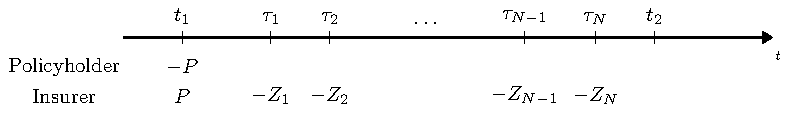
\includegraphics{_main_files/figure-latex/ins-cashflow-1.pdf}
\caption{\label{fig:ins-cashflow}Insurance Contract cash flows.}
\end{figure}

\hypertarget{non-life-insurance-pricing}{%
\section{Non-Life insurance pricing}\label{non-life-insurance-pricing}}

In insurances, the premium that the the insurer offers to the policyholder in exchange for the insurance coverage is not the same for every policyholder. The insurer evaluates the risk related to that policy and determine a ``proper'' premium taking into account risk related factors and commercial related factors. The process of \emph{pricing} corresponds in defining the set of rules for determining this ``proper'' premium \(P_i\) for a specific policyholder \(i\), given the known information on him. In the next sections I am going to better explain what ``proper'' means.

\hypertarget{compound-distribution-hypotheses}{%
\subsection{Compound distribution hypotheses}\label{compound-distribution-hypotheses}}

The first step for evaluating the stochastic process \(\left\{N, Z_1, Z_2, \dots \right\}\) is to introduce some probabilistic hypotheses. The usual hypotheses assumed are the following:

\begin{definition}[Compound distribution]
\label{def:comp-dist} \iffalse (Compound distribution) \fi{}
Let's assume that:

\begin{enumerate}
\def\labelenumi{\arabic{enumi}.}
\tightlist
\item
  for each \(n>0\), the variables \(Z_1|N=n,\ Z_2|N=n,\ \dots,\ Z_n|N=n\) are stochastically independent and identically distributed;
\item
  the probability distribution of \(Z_i|N=n, \ i\le n\) does not depend on \(n\).
\end{enumerate}

Under these hypotheses we say that:
\[
S = \sum_{i=1}^{N}{Z_i}
\]
has a compound distribution.
\end{definition}

The variable \(Z_i|N=n\) used in this definition can be interpreted as the \emph{claim severity for the \(i\)\textsuperscript{th} claim under the hypothesis that \(n\) claims occurred}. The two hypotheses provided in definition \ref{def:comp-dist} imply that the distribution of \(Z_i|N=n, \ i<n\) does not depend from \(i\) nor from \(n\). For this reason, in the following, we are going to use the notation \(Z\) to represent a random variable with the \(Z_i|N=n, \ i<n\) distribution and \(F_Z(\cdot)\) for its cumulative distribution function (i.e.~\(F_Z(z) = P(Z\le z)\)).

Let's consider the variabile \(Z_i|N>i\). We can interpret it as the \emph{claim severity for the \(i\)\textsuperscript{th} claim under the hypothesis that the \(i\)\textsuperscript{th} claim occurred}. From the hypotheses provided in definition \ref{def:comp-dist} we can obtain that also \(Z_i|N>i\) has the same distribution of \(Z_i|N=n, \ i<n\). This can be easily obtained as follows:

\begin{align}
\label{eq:z1}
P\left(Z_i \middle| N\ge i \right) & = P\left(Z_i \middle| \bigvee_{n = i}^{+\infty}{(N=n)}\right)
\\ \label{eq:z2} & =
\sum_{n=i}^{+\infty}{ \underbrace{P\left(Z_i\le z \middle| N=n\right)}_{=F_Z(z)} P\left( N = n \middle| N\ge i \right)}
\\ \label{eq:z3} & =
\sum_{n=i}^{+\infty}{ F_Z(z) P\left( N = n \middle| N\ge i \right)}
\\ \label{eq:z4} & =
F_Z(z) \underbrace{\sum_{n=i}^{+\infty}{P\left( N = n \middle| N\ge i \right)}}_{=1}
\\ \nonumber & =
F_Z(z)
\end{align}

Where:

\begin{itemize}
\tightlist
\item
  the step \eqref{eq:z1} and the step \eqref{eq:z2} are given by the fact that the event \(\{N\ge i\}\) can be decomposed as \(\{N\ge i\} = \left\{ \bigvee_{n = i}^{+\infty}{(N=n)} \right\}\) and that the events \(\{N=n\}, n\in\{i, i+1, i+2, \dots\}\) are two-by-two disjoint, so they constitute a partition of \(\{N\ge i\}\), that allows us to use the disintegrability property of the probability;
\item
  the step \eqref{eq:z3} is due to the fact that the distribution of \(Z_i\le z | N=n\) depends neither on \(i\) nor on \(n\);
\item
  the equivalence \(\sum_{n=i}^{+\infty}{P\left( N = n \middle| N\ge i \right)} = 1\) at step \eqref{eq:z4} is due to the fact that the events \(\{N=n\}, n\in\{i, i+1, i+2, \dots\}\) are a partition of \(\{N\ge i\}\).
\end{itemize}

Therefore, \(Z\) can be considered as the \emph{claim severity for a claim under the hypothesis that that claim occurred}.

\hypertarget{chap:tcc-dist}{%
\subsection{Distribution of the total cost of claims}\label{chap:tcc-dist}}

Under the hypotheses defined in definition \ref{def:comp-dist}, it is possible to obtain the full distribution of \(S\) given the distribution of \(N\) and \(Z\). In this chapter we are going to provide only the formula of the expected value \(E(S)\), but, with the same approach one can obtain all the moments.

The expected value of the total cost of claims \(E(S)\) can be obtained from the expected value of the claims count \(E(N)\) and the expected value of the claim severity \(E(Z)\) as follows:

\begin{align}
\label{eq:s1}
E(S) & = \sum_{n=0}^{+\infty}{P(N=n) \, E\left(S \middle| N = n \right)}
\\ \label{eq:s2} & =
\sum_{n=0}^{+\infty}{P(N=n) \, E\left(\sum_{i=1}^{n}{Z_i} \middle| N = n \right)}
\\ \label{eq:s3} & =
\sum_{n=0}^{+\infty}{P(N=n) \sum_{i=1}^{n}{\underbrace{E\left( Z_i \middle| N = n \right)}_{=E(Z)}}}
\\ \label{eq:s4} & =
\sum_{n=0}^{+\infty}{P(N=n) n E(Z)}
\\ \label{eq:s5} & =
E(Z) \underbrace{\sum_{n=0}^{+\infty}{n P(N=n)}}_{=E(N)}
\\ \label{eq:s6} & =
E(N)E(Z)
\end{align}

Where:

\begin{itemize}
\tightlist
\item
  the step \eqref{eq:s1} is given by the fact that the events \(\{N=0\}, \{N=1\}, \{N=2\}, \dots\) constitute a partition of the certain event \(\Omega\), that allows us to use the disintegrability property of the expected value;
\item
  the step \eqref{eq:s2} is due to the definition of \(S\);
\item
  the step \eqref{eq:s3} is due to the linearity of the expected value;
\item
  the steps \eqref{eq:s4} and \eqref{eq:s5} are due to the fact that, as assumed by the compound distribution hypotheses, \(E\left( Z_i \middle| N = n \right)\) does not depends on \(i\) and \(n\);
\item
  the step \eqref{eq:s6} is due to the definition of the expected value \(E(N)=\sum_{n=0}^{+\infty}{n P(N=n)}\).
\end{itemize}

This result tells us that, under the hypotheses of the compound distribution, it is possible to easily obtain \(E(S)\) from \(E(N)\) and \(E(Z)\). That means that we can model separately \(E(N)\) and \(E(Z)\) and, from them, obtain \(E(S)\). That result is particularly useful in personalization (paragraph \ref{chap:personalization}), because, for each individual \(i\), given the information we have on him, we can estimate his expected claim size \(E(N_i)\) and his expected claim severity \(E(Z_i)\) and obtain his expected total cost of claims as \(E(S_i) = E(N_i) E(Z_i)\).

\hypertarget{chap:risk-prem-tech-price}{%
\subsection{Risk premium and Technical Price}\label{chap:risk-prem-tech-price}}

The expected cost of claims \(E(S)\) is important because it gives us a first interpretation of what ``proper'' premium means.

\begin{definition}[Risk Premium]
\label{def:risk-premium} \iffalse (Risk Premium) \fi{} Said \(S\) the total cost of claims of a policyholder, his \emph{Risk Premium} is given by:
\[
P^{(risk)} = E(S)
\]
\end{definition}

The \emph{Risk Premium} is the premium that on average covers the total cost of claims. As mentioned above, as the coverage spans are usually short, we are not taking into account the timing of the claims so we don't discount the fact that the claims occur later than the premium payment.

It is clear that this premium, that only covers the cost of claims, is not ``proper'' in the practice.

First of all, the insurer has to cover also the expenses related to the policy (commission on sales and expenses related to the claim settlement) and the general expenses of the company. Adding the expenses, we obtain the \emph{Technical Price}.

\begin{definition}[Technical Price]
\label{def:technical-price} \iffalse (Technical Price) \fi{} Said \(S\) the total cost of claims of a policyholder and \(E\) the expenses related to his policy, his \emph{Technical Price} is given by:
\[
P^{(tech)} \ = \ E(S) + E \ = \ P^{(risk)} + E
\]
\end{definition}

Secondly, even if the policyholder would pay a premium that on average covers claims and expenses, undertaking that risk with nothing in return would not make sense for the insurer. So, to the Technical Price, some further loadings must be added, as for example risk margin and profit margin.

The result of the Technical Price with these loadings can be further modified based on business logic, as I am going to discuss later.

\hypertarget{chap:personalization}{%
\section{Modeling and Personalization}\label{chap:personalization}}

In this section we are going to better explain how pricing based on policyholder information works.

\hypertarget{chap:pricing-variables}{%
\subsection{Pricing variables}\label{chap:pricing-variables}}

Usually for every policyholder we have a certain amount of information on him that is considered relevant for his risk evaluation. This information must be reliable and observable at the moment of the underwriting of the policy.

In motor insurances, this information could be:

\begin{itemize}
\tightlist
\item
  Information on the insured vehicle: make, model, engine power, vehicle mass, age of the vehicle;
\item
  General information of the policyholder: age, sex, address (region, city, postcode), ownership of a private box where he parks the car;
\item
  Insurance specific information of the policyholder: number of claims caused in the previous years, how long he has been covered, bonus-malus class;
\item
  Policy options: amount of the maximum coverage, presence and amount of a deductible, presence of other insurance guarantees, how many drivers will drive the vehicle;
\item
  Customer information on the policyholder: how many years he has been a customer of the insurer, how many other policies he owns.
\item
  Telematic data: how many kilometers per year the policyholder travelled in the previous years, how many sharp accelerations and decelerations per kilometer the policyholder performed in the previous years.
\end{itemize}

These pieces of information are usually called \emph{pricing variables}.

We must observe that some of these variables are available for every potential customer (such as his age and address), while others are only available for policyholder that are already customers (such as telematic data that is available only if the policyholder agreed on installing on their car the device that collects this data).

Moreover, even considering the variables that are available for every customer, it is important to be aware on how reliable they are. Some of them comes from official documents (as customer age and address or bonus-malus class), but others could be declared by the customer and his statements are not easily verifiable by the insurer (as the ownership of a private box or how many drivers will drive the vehicle).

This topic of variables reliability fits in the wider framework of fraud detection. Insurance companies put a lot of effort in preventing frauds. This is done with active actions, such as documents checks and inspections, and with predictive fraud detections models. The two most common categories of frauds are underwriting frauds (such as false declaration on insurance related data) and settlement frauds (such as faking an accident). The customer information on the policyholder is usually important to predict both underwriting frauds and settlement frauds. Usually customers that have a longer relationship with the company and own many policies are less likely to commit frauds.

Regarding the topic of variables reliability, the Italian Insurance Associations (\href{https://www.ania.it/}{ANIA}) in the last years made some big steps forward by collecting in its databases a lot of information about policyholders and vehicles and making it available to insurance companies. For example, by logging in these databases it is possible, at the moment of the quote request, to retrieve useful insurance specific information such as the number of claims caused by the customer in the previous years or how long he has been covered and useful information on his vehicle such as when it has been registered or how many changes of ownership did it experienced.

One of the roles of the actuary is to understand how reliable the information on the policyholder is and to decide how to use that information.

\hypertarget{chap:pricing-variables-encoding}{%
\subsection{Pricing variables encoding}\label{chap:pricing-variables-encoding}}

Formally the pricing variables can be encoded as a vector of real numbers. \(\boldsymbol{x}_i=(x_{i1}, x_{i2}, \dots, x_{ip})\in\mathcal{X}\subseteq\mathbb{R}^p\). In the modeling framework they can be also called explanatory variables, covariates, predictors or features.

The pricing variables can be of two types:

\begin{enumerate}
\def\labelenumi{\arabic{enumi}.}
\tightlist
\item
  \emph{Quantitative variables}: variables, like policyholder age or vehicle mass, that can be easily represented as a number;
\item
  \emph{Qualitative variables}: variables, like policyholder sex or vehicle make, that represent a category and are usually represented with strings.
\end{enumerate}

The quantitative variables, with eventual transformations, are already suitable to be used.

To facilitate the use of the qualitative variables, they are usually encoded as sets of binary variables.

If a variable \(x\) has only 2 possible modalities, it can be easily encoded in a binary variable \(x'\) that assigns \(0\) to one modality and \(1\) to the other. For example, if \(x = \text{sex}\), it can be encoded this way:
\[
x' = \begin{cases}
1 & \text{if } \text{sex } = \text{ `Male'} \\
0 & \text{if } \text{sex } = \text{ `Female'}
\end{cases}
\]

In general, if a variable \(x\) has \(K\) modalities, it can be encoded in \(K-1\) binary variables \(x'_1, x'_2, \dots, x'_{K-1}\). For example, if \(x = \text{make}\) and it can have 4 possible modalities (`Fiat', `Alfa-Romeo', `Lancia', `Ferrari') it can be encoded this way:

\begin{align*}
x'_1 & = \begin{cases}
1 & \text{if } \text{make } = \text{ `Fiat'} \\
0 & \text{otherwise} \\
\end{cases}
\\
x'_2 & = \begin{cases}
1 & \text{if } \text{make } = \text{ `Alfa-Romeo'} \\
0 & \text{otherwise} \\
\end{cases}
\\
x'_3 & = \begin{cases}
1 & \text{if } \text{make } = \text{ `Lancia'} \\
0 & \text{otherwise} \\
\end{cases}
\\
\end{align*}

The variables \(x'_1\), \(x'_2\), \(x'_3\) are called dummy variables. We can observe that all the information about the make is embedded in just these 3 variables, so a fourth dummy variable that indicate the modality `Ferrari' is not needed. Indeed:

\[
\text{make } = \text{`Ferrari'} \ \Longleftrightarrow \ x'_1=x'_2=x'_3=0
\]
In table \ref{tab:dummy-variables} the dummy variable encoding is illustrated.

\begin{table}[!h]

\caption{\label{tab:dummy-variables}Dummy variables encoding.}
\centering
\begin{tabular}[t]{lccc}

\textbf{Make} & \textbf{$x'_1$} & \textbf{$x'_2$} & \textbf{$x'_3$}\\
\midrule\addlinespace
Fiat & 1 & 0 & 0\\
Alfa-Romeo & 0 & 1 & 0\\
Lancia & 0 & 0 & 1\\
Ferrari & 0 & 0 & 0\\

\end{tabular}
\end{table}

For some models it is suggested to use also the dummy variable that indicates the \(K\)\textsuperscript{th} modality. This encoding is called one-hot encoding and it is mainly used in Neural Networks. For the models considered in this paper it is preferred the \(K-1\) dummy variables encoding, so we will always consider it.

In the following, when I use the notation \(\boldsymbol{x}_i=(x_{i1}, x_{i2}, \dots, x_{ip})\), I'll always consider that the qualitative variables have been already encoded as dummy variables, so \((x_{i1}, x_{i2}, \dots, x_{ip})\in \mathcal{X} \subseteq \mathbb{R}^p\)

\hypertarget{pricing-rule-and-modeling}{%
\subsection{Pricing Rule and Modeling}\label{pricing-rule-and-modeling}}

The pricing variables are used as input of a \emph{Pricing Rule}.

\begin{definition}[Pricing Rule]
\label{def:pricing-rule} \iffalse (Pricing Rule) \fi{} A \emph{Pricing Rule} is a function \(f(\cdot)\) that from an instance of a set of pricing variables \(\boldsymbol{x}_i\in\mathcal{X}\) returns a price:

\[  
\begin{array}{rccl}
f: & \mathcal{X}      & \longrightarrow  & R_+ \\
   & \boldsymbol{x}_i & \longmapsto      & P_i \\
\end{array}
\]
\end{definition}

The process of pricing consists in defining a Pricing Rule based on observed data from the past and assumptions on the future.

The first step for defining a Pricing Rule is to model the total cost of claims \(S\) and obtain a pricing rule for the risk premium \(P^{(risk)}\).

\begin{definition}[Modeling]
\label{def:modeling} \iffalse (Modeling) \fi{} Modeling a \emph{response variable} \(Y\) means finding a function
\[r:\mathcal{X}\rightarrow \mathcal{C}\]
that, given a set of explanatory variables \(\boldsymbol{x}_i=(x_{i1}, x_{i2}, \dots, x_{ip})\in \mathcal{X} \subseteq \mathbb{R}^p\), returns the expected value of the response variable \(E(Y)\) and eventually other moments of \(Y\) or even the full distribution of \(Y\).
\end{definition}

In definition \ref{def:modeling} I used a generic \(\mathcal{C}\) as codomain of the function \(r(\cdot)\) to not specify whether the model describes just \(E(Y)\) (and so \(\mathcal{C}=\mathbb{R}\)) or something more, such as the couple \(\left( E(Y), Var(Y) \right)\) or the full distribution of \(Y\).

As we observed in section \ref{chap:tcc-dist}, under the compound distribution hypotheses, it is not needed to model directly the total cost of claims \(S\), but we can separately model \(N\) and \(Z\).

\hypertarget{response-variables-and-distributions}{%
\subsection{Response variables and distributions}\label{response-variables-and-distributions}}

Usually in statistical modeling, the response variables are seen as random variables with a distribution belonging to a specified family.

\hypertarget{chap:dist-n}{%
\subsubsection{\texorpdfstring{Distribution for the claims count \(N\)}{Distribution for the claims count N}}\label{chap:dist-n}}

The claim count \(N\) is a discrete variable with determination in \(\{0, 1, 2, 3,\dots\}\). Even if in practice the number of claims can't be arbitrarily high, \(N\) is usually modeled with distributions that give a positive probability to all the numbers in its support. One of the most common distribution used for \(N\) is the Poisson distribution.

\begin{definition}[Poisson Distribution]
\label{def:def-poisson} \iffalse (Poisson Distribution) \fi{} A random variable \(N\) with support \(\{0,1,2,3,\dots \}\) has a Poisson distribution, if its probability function is:
\[
p_N(n) = P\left( N = n \right) = e^{-\lambda}\frac{\lambda^n}{n!}, \quad \lambda>0
\]
We will indicate it with the notation \(N \sim Poisson(\lambda)\).
\end{definition}

\begin{figure}[!hbtp]

{\centering 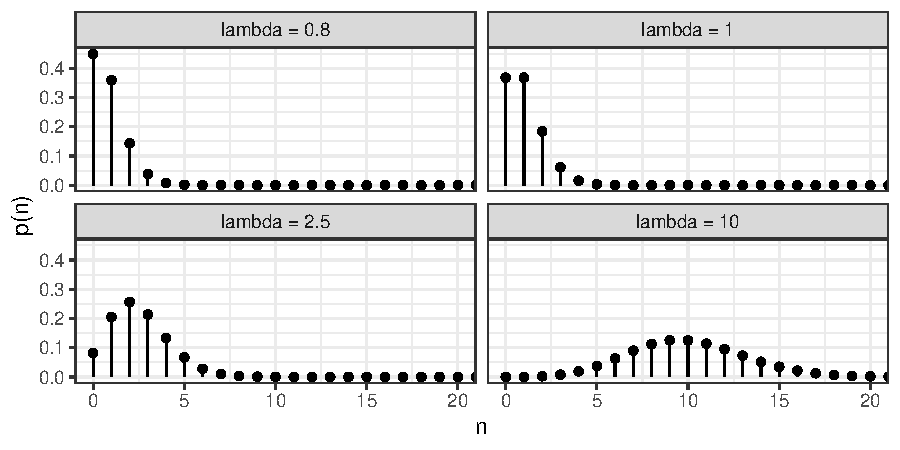
\includegraphics{_main_files/figure-latex/plot-poisson-1} 

}

\caption{Poisson distribution for some values of $\lambda$.}\label{fig:plot-poisson}
\end{figure}

The Poisson distribution is a parametric distribution that depends on only the parameter \(\lambda\). In figure \ref{fig:plot-poisson}, for different levels of \(\lambda\) the distribution is represented. These plots show how for larger values of \(\lambda\), the distribution is shifted to larger values and it is wider.

Indeed, the first two moments are:

\begin{align*}
E(N)   & = \lambda \\
Var(N) & = \lambda
\end{align*}

Thus, increasing \(\lambda\), both \(E(N)\) and \(Var(N)\) increase.

Looking to the distribution shape, we can see that:

\begin{itemize}
\tightlist
\item
  if \(\lambda<1\), the mode is in \(n=0\);
\item
  if \(\lambda=1\), \(p(0)=p(1)=\frac{1}{e}\);
\item
  if \(\lambda>1\), the mode is in a value greater than \(0\) and, as \(\lambda\) increases, the distribution assumes a bell shape similar to the Normal distribution one. The convergence to the Normal distribution can be obtained with the \emph{Central Limit Theorem}.
\end{itemize}

In non-life insurance we usually are in the case with \(\lambda<1\). E.g. the average number of claims for motor third party liability insurances in Italy, in 2018 has been 5.68\%\footnote{\href{https://www.ania.it/ricerca-avanzata/-/asset_publisher/XIyLeujL9irt/content/id/113283}{ANIA yearly statistical report for motor third party liability}}.

The property \(Var(N) = E(N)\) is an important constraint when the distribution is used in practice. It is possible that the observed data shows a different pattern. Often the observed data shows a situation where \(Var(N) > E(N)\). This phenomenon is called \emph{overdispesion}.

To address this issue it is possible to use more flexible distributions, such as Negative-Binomial distribution, or to adopt less assumptions on the response variable distribution. One common technique is the assumption of Quasi-Poisson distribution, that we will describe in chapter \ref{chap:models}.

\hypertarget{chap:exposure}{%
\subsubsection{Exposure}\label{chap:exposure}}

In section \ref{chap:non-life-ins} we said that non-life insurances usually have a fixed coverage period that usually spans for one year. Often we work with portfolios of insurances with different coverage periods. For example, this could be due to the presence of insurances born with shorter coverage periods or to the presence of insurances that has been closed earlier. Moreover, in companies data, often insurance data are collected for accounting years. This means that, if an insurance coverage \(c\) spans in two consecutive years \(a\) and \(a+1\), it is collected as two records: the couple \((c, a)\) and the couple \((c, a+1)\). This situation is quite common, as usually coverages start during the year and not all at the first of the year.

The coverage span for an insurance coverage is called \emph{exposure} and it is usually measured in years-at-risk. For instance, if an insurance coverage spans for 3 months, it corresponds to a quarter of year, so the exposure, measured in years-at-risk, is \(v=\frac{1}{4}\). The term year-at-risk comes from the fact that the policyholder exposure is a risk for the insurer, so the exposure is the period in which the insurer is exposed to the risk of paying claims.

It is natural to assume that, if a policyholder has a longer exposure, it is expected for him to experience more claims. Considering that we have to work with policies with different exposures, in order to take this aspect into account, the usual assumption taken in the following. Said \(M\) the number of claims the policyholder will experience during his period of exposure \(v\) and \(N\) the number of claims the policyholder would experience during one year, we assume \(E(M) = v E(N)\).

This assumption can be further extended if we assume that the claims come from a \emph{Poisson process}.

\begin{definition}[Counting Process]
\label{def:def-process-count} \iffalse (Counting Process) \fi{} A stocastic process \(\{N(t), t\ge0\}\) is called \textit{counting process} if:

\begin{enumerate}
\item The determination of N(t) are natural numbers \\
      $N(t) \in \{ 0, 1, 2, ... \} \ t\ge 0$
\item The process is not decreasing \\
      $s < t \Rightarrow N(s) \le N(t)$
\end{enumerate}
\end{definition}

In a counting process \(\{N(t), t\ge0\}\):

\begin{itemize}
\tightlist
\item
  \(N(t)\) can be interpreted as the number of events or arrivals that occur in the period \([0, t]\);
\item
  \(N(t) - N(s), \ s\le t\) can be interpreted as the number of events or arrivals that occur in the period \(]s, t]\). \(N(t) - N(s)\) is also called \emph{increment} of the process.
\end{itemize}

The counting process can be used to model the number of claims that occur to a specific policy.

\begin{definition}[Poisson Process]
\label{def:def-process-poisson} \iffalse (Poisson Process) \fi{} A counting process \(\{N(t), t\ge0\}\) is a \textit{Poisson process} with intensity \(\lambda\) if:

\begin{enumerate}
\item The increments of the process are stocastically independent \\
      $\forall n\ge0, \forall s_1 < t_1 \le \dots \le s_n < t_n$ \\
      $\Rightarrow \ N(t_1)-N(s_1), \dots, N(t_n)-N(s_n)$ are stocastically independent;
\item The probability of arrival in an interval is proportional to the size of the interval \\
      $\forall t\ge 0, \forall \Delta t >0 \ \Rightarrow \ P\left( N(t + \Delta t) - N(t) = 1 \right) = \lambda \Delta t + \omicron (\Delta t)$ \\
      where $\lim_{\Delta t \to 0}{\frac{\omicron(\Delta t)}{\Delta t}} = 0$
\item Multiple arrivals are excluded \\
      $\forall t\ge 0, \forall \Delta t >0 \ \Rightarrow \ P\left( N(t + \Delta t) - N(t) \ge 2 \right) = \omicron (\Delta t)$
\item Arrivals at time $0$ are almost impossible \\
      $P\left( N(0) = 0 \right) = 1 $
\end{enumerate}
\end{definition}

Under these hypotheses we obtain the following result:

\begin{theorem}[Poisson Process]
\label{thm:th-process-poisson} \iffalse (Poisson Process) \fi{} If \(\{N(t), t\ge 0 \}\) is a Poisson process with intensity \(\lambda\), then:
\[\forall t\ge 0, \forall \Delta t >0, \ \Rightarrow \ N(t + \Delta t) - N(t) \sim Poisson(\lambda \Delta t)\]
\end{theorem}

This result tells us that the distribution of the number of events in any interval \(]t, t+\Delta t]\) only depends on the size of the interval \(\Delta t\). Moreover, for the Poisson property we saw in section \ref{chap:dist-n}, we get:
\[E(N(t + \Delta t) - N(t)) = \lambda \Delta t\]

So, the expected number of arrivals is proportional to the size of the interval \(\Delta t\). The intensity of the process \(\lambda\) can be also interpreted as the expected number of claims in a unitary period.

If we assume that the claims that occur to a policy comes from a Poisson process with intensity \(\lambda\), if we observe that policy for the period \(]t, t+v]\), the claims count in that exposure period \(M\) are distributed as:
\[ M\sim Poisson(v \lambda) \]
In particular, if the observed period spans 1 year, we get:
\[ M = N \sim Poisson(\lambda) \]

\hypertarget{distribution-for-the-claim-severity-z}{%
\subsubsection{\texorpdfstring{Distribution for the claim severity \(Z\)}{Distribution for the claim severity Z}}\label{distribution-for-the-claim-severity-z}}

The claim severity \(Z\) is a continuour variable with determination in \([0, +\infty[\). As for the claims count \(N\), even if in practice it can't be arbitrarily high, it is usually modeled with distributions that give a positive probability to all the numbers in \(]0, +\infty[\). As the null claims are excluded, it is natural tu assume \(P\left( Z=0 \right) = 0\). One of the most common distribution used for \(Z\) is the Gamma distribution.

\begin{definition}[Gamma Distribution]
\label{def:def-gamma} \iffalse (Gamma Distribution) \fi{} A random variable \(Z\) with support \([0, +\infty[\) has a Gamma distribution, if its probability density function is:
\[
f_Z(z) = \frac{\rho^\alpha}{\Gamma(\alpha)}z^{\alpha-1}e^{-\rho z}, \quad \alpha > 0, \ \rho > 0
\]
where \(\Gamma(\alpha) = \int_{0}^{+\infty}{z^{\alpha - 1} e^{-z} \mathrm{d} z}\).

We will indicate it with the notation \(Z \sim Gamma(\alpha, \rho)\).
\end{definition}

\begin{figure}[!hbtp]

{\centering 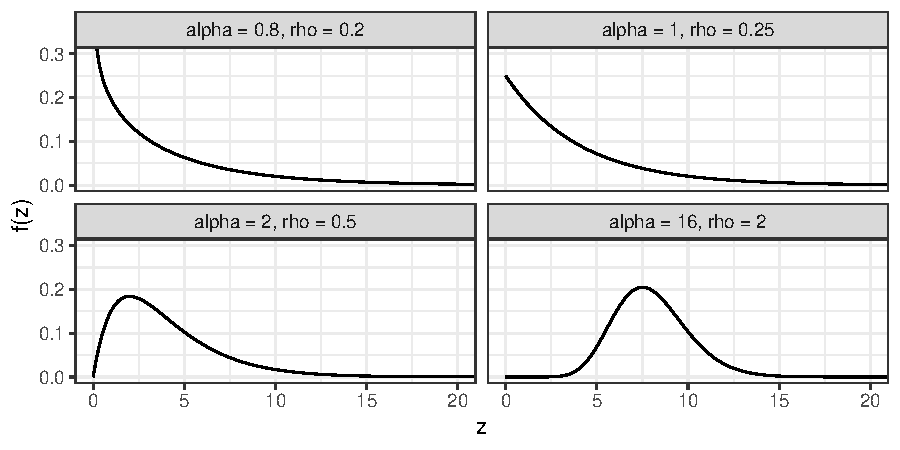
\includegraphics{_main_files/figure-latex/plot-gamma-1} 

}

\caption{Gamma distribution for some values of $\alpha$ and $\rho$.}\label{fig:plot-gamma}
\end{figure}

The Gamma distribution is a parametric distribution that depends on two parameters:

\begin{itemize}
\tightlist
\item
  \(\alpha > 0\), called shape parameter
\item
  \(\rho > 0\), called scale parameter
\end{itemize}

The first two moments of the Gamma distribution are:

\begin{align*}
E(Z)   & = \frac{\alpha}{\rho} \\
Var(Z) & = \frac{\alpha}{\rho^2}
\end{align*}

In figure \ref{fig:plot-gamma}, for different levels of \(\alpha\) and \(\gamma\) the distribution is represented. These plots show how changing the values of \(\alpha\) and \(\gamma\), the shape changes. We can see that:

\begin{itemize}
\tightlist
\item
  if \(\alpha < 1\), \(f_z(\cdot)\) is not defined in \(0\) and it has a vertical asymptote in \(z = 0\). In \(]0, +\infty]\) it is monotonically decreasing.
\item
  if \(\alpha = 1\), \(f_z(\cdot)\) starts from \(f(0) = \rho\) and then decreases monotonically. In this case, the density function becomes \(f_z(z) = \rho e^{-\rho z}\) and the distribution is also called exponential distribution.
\item
  if \(\alpha > 0\), \(f_z(\cdot)\) starts from \(f(0) = 0\), increases until the mode and then decreases.
\end{itemize}

In figure \ref{fig:plot-gamma} the first three distributions represented have the same expected value \(E(Z)=\frac{\alpha}{\rho} = 4\), but different shapes. The third and the fourth have the same variance \(Var(Z) = \frac{\alpha}{\rho^2} = 8\), but different expected values. As the shape parameter \(\alpha\) increases, the distribution assumes a bell shape similar to the Normal distribution one. The convergence to the Normal distribution can be obtained with the \emph{Central Limit Theorem}.

Another parametrization often used for Gamma distribution is obtained by using the mean \(\mu\) as a parameter:
\[
\mu = \frac{\alpha}{\rho}
\]
With this parametrization, the density function becomes:
\[
f_Z(z) = \frac{\left(\frac{\alpha}{\mu}\right)^\alpha}{\Gamma(\alpha)}z^{\alpha-1}e^{-\frac{\alpha}{\mu} z}, \quad \alpha > 0, \ \rho > 0
\]

The advantage of using the parameters \((\alpha, \mu)\) is that the link between \(E(Z)\) and \(Var(Z)\) becomes clearer:

\begin{align*}
E(Z)   & = \mu \\
Var(Z) & = \frac{1}{\alpha}\mu^2
\end{align*}

Computing the coefficient of variation we then obtain:
\[CV(Z) = \frac{\sqrt{Var(Z)}}{E(Z)} = \frac{1}{\sqrt{\alpha}}\]
This result means that, given the shape parameter \(\alpha\), the coefficient of variation is constant. As we saw for Poisson distribution, it is possible that observed data shows a different pattern. In chapter \ref{chap:models}, for Gamma distribution, we will use the parametrization based on \((\alpha, \mu)\) instead of the one based on \((\alpha, \rho)\).

Another characteristic of Gamma distribution that could be problematic in modeling claims size is that it has a light tail. This means that, as \(z\) goes to \(+\infty\), \(f_Z(z)\) aproaches \(0\) quite fast. This could lead to a poor fitting for \emph{large claims}. Other distributions with havier tails are for example the \emph{log-Normal} and the \emph{Pareto}.

\hypertarget{chap:large-claims}{%
\subsubsection{Large claims}\label{chap:large-claims}}

Modeling large claims in quite difficult in practice because usually there is not a lot of observed data on them, so it is hard to understand if they are related to some risk factors (identifiable by the pricing variables) or they happen just by chance.

First of all, to model large claims, we must define what a large claim is. What is usually done in practice is just choosing a threshold \(\bar{z}\) and considering large all the claims with a size that exceeds that threshold. The value \(\bar{z}\) must be chosen sufficiently big to consider large the claims above \(\bar{z}\), but not so big that there are not enough observed claims that exceeds \(\bar{z}\). One common choice for Motor Third Party Liability in European markets could be \(\bar{z} = 100' 000 \text{\euro}\).

\begin{definition}[Large and Attritional Claims]
\label{def:def-large-claim} \iffalse (Large and Attritional Claims) \fi{} Given a predetermined threshold \(\bar{z}\), we say that:

\begin{itemize}
\item a claim $Z$ is a \textit{large claim} if $Z > \bar{z}$
\item a claim $Z$ is an \textit{attritional claim} if $Z \le \bar{z}$
\end{itemize}

For each claim \(Z\) we call:

\begin{itemize}
\item \textit{Capped Claim Size} \\
      $Z' = \min(Z, \bar{z})$;
\item \textit{Excess Over the Threshold} \\
      $Z'' = \max(Z - \bar{z}, 0)$.
\end{itemize}
\end{definition}

In figure \ref{fig:large-claim} the \emph{Capped Claim Size} and the \emph{Excess Over the Threshold} are shown. It is easy to show that \(Z\) can be decomposed as:
\[Z = Z' + Z''\]

\begin{figure}
\centering
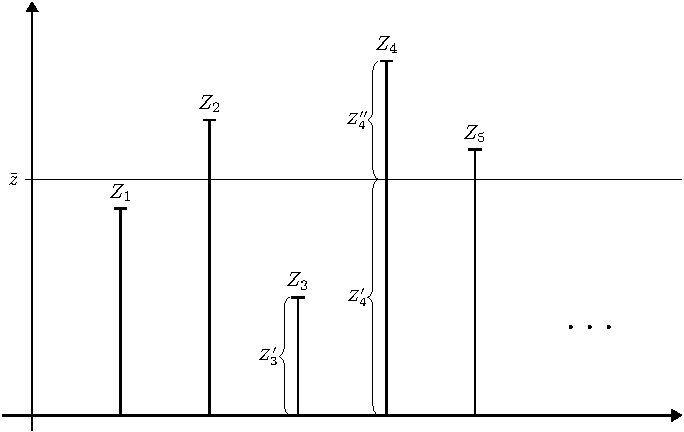
\includegraphics{_main_files/figure-latex/large-claim-1.pdf}
\caption{\label{fig:large-claim}Large claims.}
\end{figure}

Given the total number of claims \(N\), it can be decomposed as:
\[N = N^{(a)} + N^{(l)}\]

where

\begin{itemize}
\tightlist
\item
  \(N^{(a)}\) is the attritional claims count, i.e.~the number of claims with size \(Z \le \bar{z}\);
\item
  \(N^{(l)}\) is the large claims count, i.e.~the number of claims with size \(Z > \bar{z}\);
\end{itemize}

Let's indicate with \(Z_{(i)}\) the \(i\)\textsuperscript{th} in order from the smallest to the bigger. Sorting the claims we can separate the attritional claims from the large claims as follows:
\[
\underbrace{Z_{(1)}, Z_{(2)}, \dots, Z_{(N^{(a)})}}_{\text{Attritional Claims}},
\underbrace{Z_{(N^{(a)} + 1)}, Z_{(N^{(a)} + 2)}, \dots Z_{(N^{(a)} + N^{(l)})}}_{\text{Large Claims}}
\]

In order to model the large claims it is possible to use the following three decompositions of the total cost of claims \(S\):

\begin{align}
  \nonumber
  S & = \underbrace{Z_{(1)} + Z_{(2)} + \dots + Z_{(N^{(a)})}}_{\text{Attritional Claims}} +
        \underbrace{Z_{(N^{(a)} + 1)} + Z_{(N^{(a)} + 2)} + \dots Z_{(N^{(a)} + N^{(l)})}}_{\text{Large Claims}} \\
  \label{large-claim-decomposition-1}
    & = \underbrace{\sum_{i=1}^{N^{(a)}}{Z_{(i)}}}_{=S^{(a)}} +
            \underbrace{\sum_{i = N^{(a)} + 1}^{N^{(a)} + N^{(l)}}{Z_{(i)}}}_{=S^{(l)}}
    \ = \ S^{(a)} + S^{(l)} \\[12pt]
  \label{large-claim-decomposition-2}
  S & = \sum_{i=1}^{N}{Z_i}
    \ = \ \sum_{i=1}^{N}{\left(
      %\{Z_i|Z_i>\bar{z}\} I_{Z_i>\bar{z}} +
      %\{Z_i|Z_i\le\bar{z}\} I_{Z_i\le\bar{z}}
      Z_i I_{Z_i>\bar{z}} +
      Z_i I_{Z_i\le\bar{z}}
      \right)} \\[12pt]
  \label{large-claim-decomposition-3}
  S & = \sum_{i=1}^{N}{Z_i}
    \ = \ \sum_{i=1}^{N}{\left(Z'_i + Z''_i\right)}
    \ = \ \sum_{i=1}^{N}{\left(Z'_i + Z''_i I_{Z_i > \bar{z}}\right)}
\end{align}

These three decompositions of \(S\) are useful because they provide three decompositions of \(E(S)\):

\begin{align}
  \nonumber
  E(S) & = E(S^{(a)}) + E(S^{(l)}) \\
    \label{large-claim-decomposition-expected-1}
    & = E(N^{(a)}) E(Z|Z\le\bar{z}) + E(N^{(l)}) E(Z|Z>\bar{z}) \\[12pt]
  \nonumber
  E(S) & = E(N) E(Z) \\
    \nonumber
    & = E(N) \left[P(Z\le\bar{z}) E(Z|Z\le\bar{z}) + P(Z>\bar{z}) E(Z|Z > \bar{z}) \right] \\
    \label{large-claim-decomposition-expected-2}
    & = E(N) \left[\left( 1 - P(Z>\bar{z}) \right) E(Z|Z\le\bar{z}) + P(Z>\bar{z}) E(Z|Z > \bar{z})\right] \\[12pt]
  \nonumber
  E(S) & = E(N) E(Z) \\
    \label{large-claim-decomposition-expected-3}
    & = E(N) \left[E(Z') + P(Z>\bar{z}) E(Z'')\right]
\end{align}

\ref{large-claim-decomposition-expected-1}, \ref{large-claim-decomposition-expected-2} and \ref{large-claim-decomposition-expected-3} provide three approaches to model attritional and large claims.

\begin{enumerate}
\def\labelenumi{\arabic{enumi}.}
\tightlist
\item
  Looking to \ref{large-claim-decomposition-expected-1} we can model separately attritional claims and large claims. Modeling \(N^{(a)}\) and \(Z|Z\le\bar{z}\) we estimate the total cost of claims for the attritional part \(S^{(a)}\); modeling \(N^{(l)}\) and \(Z|Z>\bar{z}\) we estimate the total cost of claims for the large part \(S^{(l)}\).
\item
  Looking to \ref{large-claim-decomposition-expected-2} we can model together the claim count \(N\), and then we can model the cost of the attritional claims \(Z|Z\le\bar{z}\), the cost of the large claims \(Z|Z>\bar{z}\) and the probability to exceed the threshold \(P(Z>\bar{z})\).
\item
  Looking to \ref{large-claim-decomposition-expected-3} we can model together the claim count \(N\), and then we can model the capped claims size \(Z'\), the excess over the threshold \(Z''\) and the probability to exceed the threshold \(P(Z>\bar{z})\).
\end{enumerate}

If the large claims component weights a lot on the total cost of claims, these approaches could lead to quite different estimations of \(E(S)\). In particular, if in the observed data the number of large claims is small, it will be hard to model both \(N^{(l)}\) and \(P(Z>\bar{z})\), so the modeling process could lead to a flat or almost flat model for these components. However, with the first approach, a flat model for \(N^{(l)}\) leads to distribute the observed total cost of large claims proportionally to all the policies, while with the second and the third, a flat model for \(P(Z>\bar{z})\) leads to distribute the observed total cost of large claims proportionally to the expected number of claims \(E(N)\). So, with the first approach, a flat model brings to more solidarity between policies, while, with the second approach, a flat model could bring to an exacerbation of the differences identified by modeling \(N\).

For the second approach we must also introduce a distribution suitable for modeling \(P(Z>\bar{z})\).

\hypertarget{binomial-distribution}{%
\subsubsection{Binomial distribution}\label{binomial-distribution}}

The \emph{binomial distribution} is used to model the counting on events that occurs (successes) in a fixed amount of trials \(n\). For example we can use it to model the number of large claims withing a fixed number of \(n\) claims.

\begin{definition}[Binomial Distribution]
\label{def:def-binomial} \iffalse (Binomial Distribution) \fi{} A random variable \(Y\) with support \(\{0,1,2, \dots, n \}\) has a Binomial distribution, if its probability function is:
\[
p_Y(y) = P\left( Y = y \right) = \binom{n}{y} p^y (1-p)^{n-y}, \quad p \in [0, 1]
\]
We will indicate it with the notation \(Y \sim Binom(n, p)\).
\end{definition}

\begin{figure}[!hbtp]

{\centering 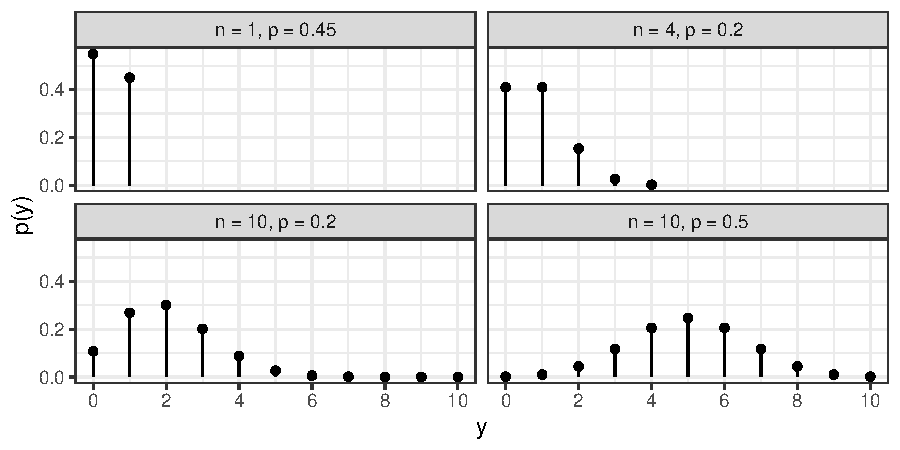
\includegraphics{_main_files/figure-latex/plot-binomial-1} 

}

\caption{Binomial distribution for some values of $n$ and $p$.}\label{fig:plot-binomial}
\end{figure}

The binomial distribution is a parametric distribution that depends on the parameters \(n\) and \(p\). \(n\) represents the number of trials, while \(p\) represents the probability for a trial to success. The assumption is that the \(n\) trials are identical, so they have all the same probability \(p\) to success. In figure \ref{fig:plot-binomial}, for different levels of \(n\) and \(p\), the distribution is represented.

The first two moments of the binomial distribution are:

\begin{align*}
E(N)   & = np \\
Var(N) & = np(1-p)
\end{align*}

If \(n = 1\), the binomial distribution assumes only the values \(1\) (with probability \(p\)) and \(0\) (with probability \(1-p\)). In this case it is also called \emph{Bernoullian distribution} and it can be used to model the indicator of an event \(I_E\).

If \(n>1\), the binomial distribution assumes a shape centered on its expected value \(E(Y)=np\) and fading for values of \(y\) that moves away from \(E(Y)\). As \(n\) increases, the distribution assumes a bell shape similar to the Normal distribution one. The convergence to the Normal distribution can be obtained with the \emph{Central Limit Theorem}.

From the binomial Distribution it is also possible to define the scaled binomial distribution by dividing its value by \(n\).

\begin{definition}[Scaled Binomial Distribution]
\label{def:def-scaled-binomial} \iffalse (Scaled Binomial Distribution) \fi{} If \(Y\sim Binom(n, p)\), and \(Y' = \frac{Y}{n}\), we will say that \(Y'\) has a \textit{Scaled Binomial Distribution} and we will indicate it with the notation \(Y' \sim Binom(n, p)/n\).

The support of \(Y'\) is \(\{0, \frac{1}{n}, \frac{2}{n}, \dots, 1 \}\) and its probability function is:
\[
p_{Y'}(y') = P\left( Y' = y' \right) = \binom{n}{ny'} p^{ny'} (1-p)^{n-ny'}, \quad p \in [0, 1]
\]
\end{definition}

In chapter \ref{chap:models} we will use the Scaled Binomial Distribution.

In non-life insurance pricing, the binomial distribution can be used to model the probability for a claim to have specific characteristics. For example we can use it to model the probability that a certain claim is a large one \(P(Z>\bar{z})\) in order to model separately attritional claims severity \(\{Z|Z\le\bar{z}\}\) and large claims severity \(\{Z|Z>\bar{z}\}\), as we have seen in section section \ref{chap:large-claims}.

Another example is the decomposition between claims with only material damages and claims with also bodily injuries. Modeling separately these two components is useful because they usually have a different distribution for the claim size.

As for large claims we can decompose \(S\) in the following two ways:

\begin{align}
  \nonumber
  E(S) & = E(S^{(things)}) + E(S^{(inj)}) \\
    \label{inj-claim-decomposition-expected-1}
    & = E(N^{(things)}) E(Z|\bar{J}) + E(N^{(inj)}) E(Z|J) \\[12pt]
  \nonumber
  E(S) & = E(N) E(Z) \\
    \nonumber
    & = E(N) \left[P(\bar{J}) E(Z|\bar{J}) + P(J) E(Z|J) \right] \\
    \label{inj-claim-decomposition-expected-2}
    & = E(N) \left[\left( 1 - P(J) \right) E(Z|\bar{J}) + P(J) E(Z|J)\right]
\end{align}

where:

\begin{itemize}
\tightlist
\item
  \(N^{(things)}\) is the number of claims with only material damages;
\item
  \(N^{(inj)}\) is the number of claims with injuries;
\item
  \(J\) is the event that represent that a specific claim presents injuries; such as \(Z\) is a representative for \(Z_1, Z_2, \dots, Z_N\), \(J\) is a representative for \(J_1, J_2, \dots, J_N\).
\end{itemize}

Combining this decomposition with what we have seen in large claims decomposition, we can further develop our decomposition taking into account both the presence or absence of injuries and the occurrence or not of a large claim. One example could be:

\begin{align*}
E(S) & = E(N) \left[\left( 1 - P(J) \right) E(Z|\bar{J}) + P(J) E(Z|J) \right] \\[4pt]
  & = E(N) \left\{ \right. \\
  & \qquad \left( 1 - P(J) \right) E(Z|\bar{J}) \\
  & \qquad + P(J) \left[ \right. \\
  & \qquad \qquad P(Z \le \bar{z} | J) E\left( Z \mid Z\le \bar{z} \land J \right) \\
  & \qquad \qquad + P(Z < \bar{z} | J) E\left( Z \mid Z < \bar{z} \land J \right) \\
  & \qquad \left. \right] \\
  & \quad \left. \right\}
\end{align*}

This way, we are decomposing only the claims with injuries between attritional and large. That makes sense because claims that don't produce injuries usually have small severities.

\hypertarget{model-fitting-and-data-available}{%
\subsection{Model fitting and data available}\label{model-fitting-and-data-available}}

Once we have chosen how to decompose \(S\), we have to model the response variables needed for that decomposition (\(N\), \(Z\), \(I_J\), \ldots) with the explanatory variables. Thus we have to estimate a function \(r:\mathcal{X}\rightarrow \mathcal{C}\) as defined in \ref{def:modeling}.

In order to estimate \(r(\cdot)\) we have also to take some assumptions on the distribution of the response variable and on the shape of \(r(\cdot)\). We will call \emph{model} a set of assumptions on the response variable and on the shape of \(r(\cdot)\). We will discuss some of the most widespread models for claims count and claims severity in chapter \ref{chap:models}.

Defined the model, we have to estimate it using observed data. In general, to model a response variable \(Y_i\) with the explanatory variables \(\boldsymbol{x}_i=(x_{i1}, x_{i2}, \dots, x_{ip})\in \mathcal{X} \subseteq \mathbb{R}^p\), the observed data is in the form:
\[
\mathcal{D} = \left\{(\boldsymbol{x}_1, w_1, y_1), \ (\boldsymbol{x}_2, w_2, y_2), \ \dots, \ (\boldsymbol{x}_i, w_i, y_i), \ \dots, \ (\boldsymbol{x}_n, w_n, y_n)\right\}
\]
where:

\begin{itemize}
\tightlist
\item
  \(n\) is the number of observations in the dataset;
\item
  \(\boldsymbol{x}_i\in \mathcal{X} \subseteq \mathbb{R}^p\) is the set of explanatory variable for the observation \(i\);
\item
  \(w_i\) is the weight for the observation \(i\);
\item
  \(y_i\in \mathcal{Y}\ \subseteq \mathbb{R}\) is the realization of the response variable \(Y_i\) for the observation \(i\).
\end{itemize}

What an observation is, depends on the variable we are modeling. For instance:

\begin{itemize}
\tightlist
\item
  If we are modeling the yearly claim count \(N_i\), each observation could be a policy (or a couple (policy, accounting year)), the weights could be the exposures \(v_i\) and the realizations of response variables could be the number of observed claims for that policy (or couple (policy, accounting year)).
\item
  If we are modeling the claim severity \(Z_j\), each observation could be a claim \(j\), the weights could all be \(1\) and the realizations of response variables could be the observed cost for the claim \(j\). It is also possible to model the claim severity taking into account the total cost of claims for the policy \(S_i = \sum_{j=1}^{N_i}{Z_j}\). In this case, each observation would be a policy \(i\), the weights would be the number of claims for each policy \(n_i\) and the realizations of response variables would be the total observed cost for the claims of the policy \(i\).
\item
  If we are modeling the occurrence of injuries in a claim \(I_{Jj}\), each observation could be a claim \(j\), the weights could be all \(1\) and the realizations of response variables could be an indicator that assume the value \(1\) if the claim \(j\) caused injuries and \(0\) otherwise. As for the claim severity, we can also aggregate data for policy, so each observation would be a policy \(i\), the weights would be the number of claims \(n_i\) for the policy \(i\) and the realizations of response variables would be the number of claims that caused injuries among the claims of the policy \(i\).
\end{itemize}

In each of these cases, \(y_i\) is seen as a realization of the random variable \(Y_i\). With an inferential process we obtain estimations on \(Y_i\) disctribution based on observations of their realizations \(y_i\).

\hypertarget{settlement-process-and-ibnr}{%
\subsubsection{Settlement process and IBNR}\label{settlement-process-and-ibnr}}

One of the challenges in non-life insurance pricing is that obtaining the observed data is not so straightforward. In many insurance coverages, such as MTPL, the settlement process could last many years, so, if we want to develop models using data from recent years, not all the information is available. To better understand this aspect we have to discuss how the settlement process works.

In figure \ref{fig:settlement-process} the settlement process for a claim is represented. At time \(t_1\) the insured event (e.g.~an accident) occurs. From this moment a liability for the insurer emerges, even if the insurer has not been notified yet. This liability is called \emph{Outstanding Loss Liability}. In \(t_2\) the claim in reported and the insurance is notified about the occurrence of the event. From this moment the settlement process starts. This process consists in evaluating the event and understanding the responsibilities of the parts and the entity of the damage. During this process, controversies between the parts can emerge and, in particular if injuries occurred, the damage evaluation can takes a lot of time. When the situation in clear and everything is defined, the claim is settled and the liabilities are payed. In \(t_3\) we have the settlement and in \(t_4\) the claim is closed. In is possible that \(t_4=t_3\), but in general it is not always the case. If the settlement process takes a long time and the insurer already knows he will have to pay something, he can pay some partial payments during the period \([t_2, t_3]\). These intermediate payments are payed at times \(\tau_1, \tau_2, \dots, \tau_n \in [t_2, t_3]\). It is also possible that a claim is opened and then gets closed without any payment. After the closing (\(t_4\)) it is also possible that a claim is reopened and that more payments emerge.

\begin{figure}
\centering
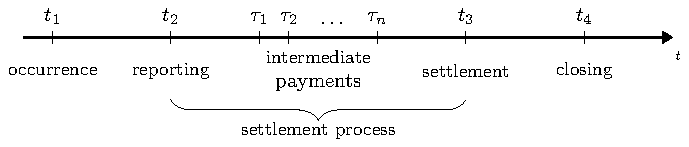
\includegraphics{_main_files/figure-latex/settlement-process-1.pdf}
\caption{\label{fig:settlement-process}Claim timeline.}
\end{figure}

From the moment the claim is reported (\(t_2\)), the insurer estimates how much he is going to pay for that claim and he allocates that sum in a reserve. As new information emerges and some payments are settled, the reserve is updated. The aim for this reserve is to have a best estimate for the future payments for the claims already emerged. As the claim gets settled, the sum between the payed and the reserved converges to the final cost of the claim.

From this description emerges that:

\begin{itemize}
\tightlist
\item
  In the period \(]t_1, t_2[\) the insurer has an outstanding loss liability for an event that has not been reported yet; in this case we will talk about \emph{Incurred But Not Yet Reported} claim (\emph{IBNyR}).
\item
  In the period \([t_2, t_3[\) the insurer has an outstanding loss liability for an event that has been reported, but has not been totally settled yet, so that liability is just an estimate; in this case we will talk about \emph{Incurred But Not Enough Reported} claim (\emph{IBNeR}).
\end{itemize}

\hypertarget{model-fitting-with-available-data}{%
\subsubsection{Model fitting with available data}\label{model-fitting-with-available-data}}

The IBNyR and IBNeR issue is particularly challenging when we have to perform a risk evaluation at a specific time \(t\). In general \(t_1, t_2,\dots\) are not known a priori, so we don't know if in the future more claims for accidents occurred in the past will be reported and we don't know if the ones that are already reported will experience a revaluation. That means that, in general, when we model \(N\) and \(Z\) at a specific time \(t\), we can't observe the total number of claims occurred to each policy \(n_i\) and the payments for each claim \(z_j\). What we can use is:

\begin{itemize}
\tightlist
\item
  \(n_i^{(t)} = n_i^{(\text{reported in } t)}\)\\
  where:

  \begin{itemize}
  \tightlist
  \item
    \(n_i^{(\text{reported in } t)}\) is the number of reported claims in \(t\) for the policy \(i\);
  \end{itemize}
\item
  \(z_j^{(t)} = z_j^{(\text{payed in }t)} + z_j^{(\text{reserved in } t)}\)\\
  where:

  \begin{itemize}
  \tightlist
  \item
    \(z_j^{(\text{payed in }t)}\) is the amount already payed in \(t\) for the claim \(j\);
  \item
    \(z_j^{(\text{reserved in } t)}\) is the amount reserved in \(t\) for the claim \(j\).
  \end{itemize}
\end{itemize}

When we use this data for modeling the total cost of claims we must be particularly aware on what we are using. In general:

\begin{align*}
n_i^{(t)} & \ne n_i \\
z_j^{(t)} & \ne z_j
\end{align*}

The common case is that \(n_i^{(t)} < n_i\) and \(z_j^{(t)} < z_j\). If we used \(n_i^{(t)}\) and \(z_j^{(t)}\) without any correction, we would underestimate both \(E(N)\) and \(E(Z)\), obtaining a distorted estimate for \(E(S)\).

To tackle these problems what is usually done is fitting the models for \(S_i\) with \(n_i^{(t)}\) and \(z_j^{(t)}\) and then apply a flat corrective coefficients \(\alpha\) to \(\widehat{E(S_i)}\) based on an aggregated estimate of \(E(S)\) that takes into account the long settlement process.

An estimate for the expected total cost of claims for a generic policy in the portfolio \(E(S)\) can be obtained with techniques based on runoff triangles, such as the \emph{Chain Ladder}. These techniques are based on projecting the cost of claims already emerged to the final total cost of claims. We are not going to discuss these techniques in this thesis. We just have to know that these techniques provide us with an estimate for \(E(S)\). Let's call it \(\widehat{E(S)}^{CL}\). This estimate does not depend on explanatory variables; it is a sort of average total cost of claims for the policies in the portfolio.

Meanwhile, with the available data \(n_i^{(t)}\) and \(z_j^{(t)}\), the fitting for all the models needed in the decomposition of \(S\) is performed and, for each policy \(i\in\{1, 2, \dots, n\}\) for \(E(S_i)\) is obtained. Let's call it \(\widehat{E(S_i)}'\). As we used the data available in \(t\) that comes from claims not totally settled, \(\widehat{E(S_i)}'\) is a distorted estimate for \(E(S_i)\).

We can then balance the estimates \(\widehat{E(S_i)}'\) with \(\widehat{E(S)}^{CL}\) by computing:
\[
\alpha = \frac{n}{\sum_{i=1}^{n}{\widehat{E(S_i)}'}} \widehat{E(S)}^{CL}
\]
and applying to the estimates as follows:
\[
\widehat{E(S_i)} = \alpha \ \widehat{E(S_i)}'
\]

We will call \(\widehat{E(S_i)}\) rebalanced estimates.

The property of these balanced estimates is that on average they point to \(\widehat{E(S)}^{CL}\):

\begin{align*}
\frac{\sum_{i=1}^{n}{\widehat{E(S_i)}}}{n} & = \frac{\sum_{i=1}^{n}{\alpha\widehat{E(S_i)}'}}{n} \\
& = \alpha\frac{\sum_{i=1}^{n}{\widehat{E(S_i)}'}}{n} \\
& = \frac{n}{\sum_{i=1}^{n}{\widehat{E(S_i)}'}} \widehat{E(S)}^{CL} \frac{\sum_{i=1}^{n}{\widehat{E(S_i)}'}}{n} \\
& = \widehat{E(S)}^{CL}
\end{align*}

So, if \(\widehat{E(S)}^{CL}\) is a unbiased estimator for \(E(S)\), we obtain:
\[
E\left( \frac{\sum_{i=1}^{n}{\widehat{E(S_i)}}}{n} \right)
= E\left( \widehat{E(S)}^{CL} \right)
= E(S)
\]

This procedure can be further developed by balancing not directly the total cost of claims \(E(S)\), but its components. For example, we could separately balance the total cost of claims that only caused damage to things and the total cost of claims that caused injuries. This separation in components can lead to a more precise estimate because usually claims that caused injuries have a slower settlement process so they will have a higher corrective coefficient \(\alpha\).

If the dataset contains policies from many years and during last years a relevant change in the portfolio risk mixture happened, it is also possible to compute \(\alpha\) not with all the \(n\) policies of the dataset, but only with the policies from the last year of the dataset.

The fact that the final estimates \(\widehat{E(S_i)}\) are rebalanced on \(\widehat{E(S)}^{CL}\) means that the explanatory variables effects estimated with \(n_i^{(t)}\) and \(z_j^{(t)}\) are used just as relative effects and not absolute ones. For instance, if the model says that young people have an expected total cost of claims \(\widehat{E(S_i)}'\) that is two times the old people one, that relative coefficient 2 will be kept also in the balanced estimate \(\widehat{E(S_i)}\).

For this reason, in practice, often the modeling is considered composed in 2 parts:

\begin{enumerate}
\def\labelenumi{\arabic{enumi}.}
\tightlist
\item
  \emph{Tariff Requirement} (or \emph{Fabbisogno Tariffario}): the estimate of \(\widehat{E(S)}^{CL}\) by aggregated data;
\item
  \emph{Personalization}: the estimate of \(\widehat{E(S_i)}'\) and the relative coefficients.
\end{enumerate}

The techniques used for \emph{Tariff Requirement} are employed also to estimating the general liability position for the company. This information is particularly important and it is reported in the company financial statement.

\hypertarget{beyond-technical-pricing}{%
\section{Beyond technical pricing}\label{beyond-technical-pricing}}

In section \ref{chap:risk-prem-tech-price} we defined:

\begin{itemize}
\tightlist
\item
  the \emph{Risk Premium}\\
  \(P^{(risk)} = E(S)\)
\item
  the \emph{Technical Price}\\
  \(P^{(tech)} = E(S) + E\)
\end{itemize}

In section \ref{chap:personalization} we described how the risk premium can be estimated. In this thesis we are not going to deal with the estimate of the expenses.

In this section we are going to discuss what the \emph{Tariff} and the \emph{Offer Price} are and which are the further needs that the offer should satisfy. The following description is referred to MTPL insurance in the Italian market. Most of the comments we make can be applied to other motor coverages too.

\hypertarget{tariff-and-offer-price}{%
\subsection{Tariff and Offer Price}\label{tariff-and-offer-price}}

The \emph{Tariff} is the official price for the policy. Over the cost of claims and the expenses, it must include all the loadings for cost of capital and profits. The tariff has a particular importance because it is subjected to strict regulations and it must be approved by the supervisory authority, that in Italy is the IVASS (Istituto per la vigilanza sulle Assicurazioni).

In section \ref{chap:pricing-variables} we described some of the explanatory variables that can be used to build the technical price. For technical pricing there are no constraints because it is used only for internal monitoring and the final price proposed to the client does not directly depends on it. However, some of the variables used for technical pricing can't be used in tariff. In particular, the regulations say that companies can't discriminate clients based on sex, ethnic group, religion or place of birth. Thus, for example, even if from statistical data we see that women usually experience less claims than men, we can't discriminate men by offering them a higher price. Moreover, some variables have constraints on tariff coefficients. For example, in MTPL insurance, the bonus-malus class is strongly regulated. Every company must recognize the bonus-malus class matured by clients (even if they matured them with other companies) and the coefficients of this variable must be monotonically increasing, i.e.~a lower class must correspond to a better tariff. We remind that in the Italian bonus-malus system the lower the class the better the premium. Another tariff constraint is that for some coverage, such as MTPL, the insurer has an obligation to contract. That means that whoever the client is, independently to how risky he is, the company must offer a premium and, if the client accepts, the company must underwrite the insurance contract. In this context, if the company offers an unreasonably high premium, it could fall in an attempt to avoiding the obligation to contract. For this reason, the tariff can't be arbitrarily high and must contemplate a maximum premium. To be sure that all the costraints has been respected, the tariff, before entering in production, must follow a strict approval process.

To make the offer price more flexible and to facilitate business competition, the supervisory authority allows insurance companies to sell policies not to the tariff price, but to the price obtained subtracting from it a discount \(D_i\ge0\). The premium obtained this way is called \emph{Offer Price}.
\[
P^{(\text{offer})}_i = P^{(\text{tariff})}_i - D_i
\]

That means that, for the offer price to adequately cover the cost of claims and expenses, the tariff must include a loading for discounting. This loading for discounting, called \emph{discounting flexibility}, can be partially spended by the agent and partially by the insurance company itself. The discounts can be changed over time in a much more agile way than the tariff. For example in Italy, during the Spring 2020 Covid19 crisis, many companies introduced measures to support clients needs with important discounts on both new business and renewal. From a technical point of view, these discounts have been funded by the remarkable decrese on claim frequency due to the traffic decreasing. Discount measures like these are welcomed by the supervisory authority because they promote business competition and lead to lower prices for consumers.

\hypertarget{commercial-price}{%
\subsection{Commercial price}\label{commercial-price}}

Both tariff and offer price must be based not only on technical logic, but also on commercial one. They are determined with a process of \emph{Price Optimization}. The final goal for a company is to maximize profits this year and in the next ones, so the objective of commercial pricing must be obtaining the optimal price to reach this goal. Maximizing profits is a quite generic goal and can't be easily expressed as an analytical optimization problem. For this reason the pricing choices can be guided by the business strategy that can be translated in specific \emph{Key Performance Indicators} (KPI) that have to be optimized. In this optimization framework, the technical price can be seen as an estimate of the expected cost related to the policy. Knowing the costs it is possible to tune the final premium by working on margins.

The components that act on price optimization can be addressed to:

\begin{enumerate}
\def\labelenumi{\arabic{enumi}.}
\tightlist
\item
  \emph{technical pricing};
\item
  \emph{client expectation};
\item
  \emph{business strategy}.
\end{enumerate}

We already extensively covered technical pricing in previous chapters.

Client expectation is basically the price that the client is willing to pay for the specific product. Here the basic idea is that if the client would pay a premium much higher than the technical one, it wouldn't make sense for the company to sell him the product at technical price. This is a big opportunity to gain margins. To analyze client expectation, what is usually done is:

\begin{itemize}
\tightlist
\item
  for new business modeling his conversion probability
\item
  for renewal business modeling his retention probability.
\end{itemize}

For example some guarantees or some options are perceived by the clients as being really worth even if their technical price is not so high. The perception of the client depends also on the competitors pricing and how easy comparing offers from different companies is. In the last years, in the Italian market, the development of aggregators has made much easier for consumers to compare offers from different companies, increasing the competition and the attention on pricing. Anyway, if a company is able to differentiate itself from the others and to make its product been perceived as more valuable, it can sell it at a higher price than other companies. For example this can be achived by improving customer service and customer experience.

If the technical price and the conversion probability function are given, finding the optimal price for a policy can be expressed as an analytical optimization problem. However, to find the optimal price, one should also take into account that usually policies are not sold alone, but in packages of guarantees. With a wider vision, a business strategy could be selling MTPL policy with almost no margins if it allows to sell other guarantees with higher margins. Moreover, as the aim is not to be profitable this year, but also in the following ones, the company should also consider the \emph{lifetime value} of the client. Indeed, a satisfied client will also stipulate other contracts in the future and can bring to the company other clients from his connections. So, selling a policy with small margins today can lead to high margins tomorrow in other policies.

The business strategy could also contemplate being more aggressive on certain targets of client and less on others. For example, if the company is particularly strong in certain regions, it could make sense for it to push in that region to further increase its market share. Vice versa, in regions where the company doesn't sell much, it could be safer not to push too much and to be more careful. In a risk management framework, this can be also interpreted as introducing a further risk margin for clusters where there isn't enough observed data and the lack of information brings to more uncertainty. An aggressive pricing can also make sense for a young company that is growing and it is not supposed to be profitable from the first years. From a marketing point of view this strategy can increase the brand awareness by the clients and can strengthen the company image.

Anyway, a company can't arbitrarily discount policies because an excess in discounting could cause severe drawbacks on a financial perspective. Therefore, an insurance company must always respect the solvency constraints defined by the supervisory authority to safeguard itself from bankruptcy. The company solvency is essential to protect all the stakeholders, that are both the clients and the investors.

\hypertarget{the-actuary-role}{%
\section{The actuary role}\label{the-actuary-role}}

In this technical and commercial pricing framework, the actuary is the one that conduct the analysis and define the pricing rules. The \emph{International Actuarial Association} (IAA) describes the actuaries are ``highly qualified professionals who analyze the financial impact of risk for organizations like insurers, pensions fund managers, and more'' and it states that their work ``requires a combination of strong analytical skills, business knowledge, and understanding of human behavior''.\footnote{\href{https://www.actuaries.org/iaa/IAA/About_the_IAA/About_Actuaries/About\%20Actuaries.aspx}{IAA, About Actuaries}}

First of all, the actuary must master the main statistical and data science techniques used to develop model for technical pricing. On this field, in the last years, the development of machine learning and high performance computing has permitted a huge development of technical pricing allowing actuaries to use much more complex variables and models. However, the actuary does not have just to be en expert in statistics and machine learning. He must be also able to interpret the results he gets with his models and use his expertise to understand if the results he gets are fine for future predictions. As we already mentioned, the pricing rules will be used for policies that will be sold in the future, so they have to be defined with a mixture of observation of the past and assumptions on the future. In addition, sometimes it is needed to define price for clusters where the company have no historical data. This can happen when a company is expanding to new customers for example by opening new selling channels or by pushing in regions where its market share is quite small. Furthermore, the lack of historical data can be due to the full sector evolution. For example, in these years, new vehicles, such as electric cars and cars with Advanced Driver-Assistance Systems (ADAS), are spreading. As these vehicles didn't exist in the past, historical data doesn't exist. So, finding the proper pricing is challenging. From the company point of view, positioning with a competitive pricing on these segments is important for future business, but the risk must be properly evaluated. For these kind of tasks, the actuary must have a deep domain knowledge on the field.

In the last years, the increase of competition brought to an increase in commercial price importance. Now most of the companies build their own conversion and retention probability models and they are developing more complex business strategies. In this context, it is fundamental for the actuary to understand the clients behaviors, in order to optimize tariff and offer price. The importance for commercial pricing implicate that the technical pricing must not be conducted independently from commercial pricing. Even in companies where the technical pricing and the commercial pricing are carried out by two separate teams, the two teams have to collaborate and coordinate together. This need has some relevant implications on how technical pricing is conducted that we will further discuss in section \ref{chap:actuary-importance}.

--\textgreater{}

\hypertarget{chap:models}{%
\chapter{\texorpdfstring{\textbf{Statistical models for Non Life Insurance Pricing}}{Statistical models for Non Life Insurance Pricing}}\label{chap:models}}

\minitoc  

\chaptermark{Statistical models for Non Life Insurance Pricing}

In this chapter we are going to illustrate some of the most widespread models for technical pricing. For each model we are going to describe its benefits and drawbacks and in section \ref{chap:actuary-importance} we will compare them by discussing how they fit the pricing needs.

\hypertarget{statistical-models}{%
\section{Statistical Models}\label{statistical-models}}

In this section we will start by describing the Generalized Linear Model (GLM), that is the most employed model in technical pricing, to then present some of its advancements: the Elastic Net and the Generalized Additive Model (GAM). After this description, we will also present the Gradient Boosting Machine (GBM), that is one of the most effective general purpose machine learning models. This allows us to have a comparison between GLM based models and general purpose machine learning models.

\hypertarget{glm}{%
\subsection{GLM}\label{glm}}

\hypertarget{chap:linear-exp-families}{%
\subsubsection{Linear Exponential Families}\label{chap:linear-exp-families}}

One of the GLM assumptions is that the response variables belong to a \emph{Linear Exponential Family}. In this section we are going to explain what a linear exponential family is and which distributions fit its definition.

\begin{definition}[Linear Exponential Family]
\label{def:linear-exp-family} \iffalse (Linear Exponential Family) \fi{} A Linear Exponential Family \(\mathcal{F}\) is a parametrical family of probability distributions with density function (or probability function in the discrete case) that can be expressed in the form:
\[
f(y; \theta, \lambda) = \exp{\left\{ \frac{y\theta-b(\theta)}{\lambda} \right\}} c(y,\lambda), \quad y\in \mathcal{Y}\subseteq\mathbb{R}
\]
where:

\begin{itemize}
\item $\theta\in\Theta\subseteq\mathbb{R}$ is called \textit{canonical parameter};
\item $\lambda\in\Lambda\subseteq]0, +\infty[$ is called \textit{dispersion parameter};
\item $b: \Theta \rightarrow \mathbb{R}$ is a real function called \textit{cumulant function};
\item $c: (\mathcal{Y}, \Lambda) \rightarrow [0, +\infty[$ is a real function;
\item $\Theta$ is a non degenerate interval, i.e. $\text{int}\Theta$ is not empty.
\end{itemize}
\end{definition}

An exponential family \(\mathcal{F}\) is characterized by the elements \(\left( \Theta, b(\cdot), \Lambda, c(\cdot, \cdot) \right)\). By properly choosing the sets \(\Theta, \Lambda\) and the functions \(b(\cdot), c(\cdot, \cdot)\), it is possible to obtain many useful families.

It can be easily shown that the families Normal, Poisson, Gamma and Binomial are exponential families. In table \ref{tab:exp-families} the characterizations for these exponential families are reported.

\begin{table}[!h]

\caption{\label{tab:exp-families}Some Linear Exponential Families.}
\centering
\begin{tabular}[t]{lcccccc}
\toprule
\textbf{Distribution} & \textbf{Notation} & \textbf{$\Theta$} & \textbf{$\theta$} & \textbf{$\Lambda$} & \textbf{$\lambda$} & \textbf{$b(\theta)$}\\
\toprule\addlinespace
Normal & \makecell[c]{$N(\mu, \sigma^2)$,\\$\mu\in\mathbb{R}$ \\ $\sigma \in ]0, +\infty[$} & $\mathbb{R}$ & $\mu$ & $]0, +\infty[$ & $\sigma^2$ & $\frac{\theta^2}{2}$\\
\addlinespace\hline\addlinespace
Poisson & \makecell[c]{$Poisson(\mu)$,\\$\mu \in ]0, +\infty[$} & $\mathbb{R}$ & $\log{(\mu)}$ & $\left\{1\right\}$ & $1$ & $e^{\theta}$\\
\addlinespace\hline\addlinespace
Gamma & \makecell[c]{$Gamma(\alpha, \mu)$,\\$\alpha \in ]0, +\infty[$ \\ $\mu \in ]0, +\infty[$} & $]-\infty, 0[$ & $-\frac{1}{\mu}$ & $]0,+\infty[$ & $\frac{1}{\alpha}$ & $-\log{\left(-\theta\right)}$\\
\addlinespace\hline\addlinespace
\makecell[l]{Scaled\\Binomial} & \makecell[c]{$Binom(n, p)/n$,\\$n\in\mathbb{N}$ \\ $p\in]0,1[$} & $\mathbb{R}$ & $\log{\left(\frac{p}{1-p}\right)}$ & $\left\{\frac{1}{n}\right\}$ & $\frac{1}{n}$ & $\log\left(1+e^{\theta}\right)$\\
\bottomrule
\end{tabular}
\end{table}

The distributions that belong to an exponential family have many useful properties. For example they are provided with all the moments and their moments can be obtained using the derivatives of the cumulative function \(b(\cdot)\). If \(Y\) is a random variable with distribution belonging to an exponential family \(\mathcal{F}\) with parameters \(\theta, \lambda\), its first two moments are:

\begin{align}
\label{eq:exp-fam-expected-value}
E(Y)   & = b'(\theta) \\
Var(Y) & = \lambda b''(\theta)
\end{align}

As, within a specified family, the parameters \(\theta\) and \(\lambda\) determine a distribution, in practical problems the object of estimation will be the couple \((\theta, \lambda)\). In many problems it is natural to consider distributions from a linear exponential family where the dispersion parameter can be expressed as \(\lambda = \frac{\phi}{\omega}\), where \(\omega>0\) is a known \emph{weight} and \(\phi>0\) is a parameter that we will keep calling \emph{dispersion parameter}. In this case, the density of probability function depends on the parameters \(\theta\) and \(\phi\) and will be expressed as:
\[
f(y; \theta, \phi, \omega) = \exp{\left\{ \frac{\omega}{\phi} \left[y\theta - b(\theta) \right] \right\}} c(y, \phi, \omega), \quad y\in \mathcal{Y}\subseteq\mathbb{R}
\]

In this case the parameters \(\theta\) and \(\phi\) will be object of estimation, while \(\omega\) is an already known value. As we will see later, this representation allows us to consider as known weights:

\begin{itemize}
\tightlist
\item
  the exposure \(v\) in the Poisson distribution;
\item
  the number of trials \(n\) in the Binomial distribution.
\end{itemize}

\hypertarget{model-assumptions}{%
\subsubsection{Model assumptions}\label{model-assumptions}}

Let's assume that, for \(n\) statistical units, the observations \(\mathcal{D} = \left\{ (\boldsymbol{x}_1, \omega_1, y_1), \dots, (\boldsymbol{x}_n, \omega_n, y_n) \right\}\) are available, where \(\boldsymbol{x}_i\) is a vector of explanatory variables determinations, \(\omega_i\) is a known weight and \(y_i\) is the response variable determination. \(\boldsymbol{x}_i, \omega_i, y_i\) are all real numbers. The vector \(\boldsymbol{y} = (y_1, \dots, y_n)^t\) is considered a determination of the response random vector \(\boldsymbol{Y} = (Y_1, \dots, Y_n)^t\).

In GLM we assume that:

\begin{enumerate}
\def\labelenumi{\arabic{enumi}.}
\tightlist
\item
  The response variables \(Y_1, \dots, Y_n\) are stochastically independent and with probability distribution belonging to a same linear exponential family; i.e.~the probability distribution of \(Y_i\) has density function (or probability function in the discrete case) that can be expressed as:
  \[
  f(y_i; \theta_i, \phi, \omega_i) = \exp{\left\{ \frac{\omega_i}{\phi} \left[y_i\theta_i - b(\theta_i) \right] \right\}} c(y_i, \phi, \omega_i), \quad y_i\in \mathcal{Y}\subseteq\mathbb{R}
  \]
  We highlight that only \(\theta_i\) and \(\omega_i\) depend on \(i\), while the dispersion parameter \(\phi\) is the same for all the observations.
\item
  The explanatory variables determinations vector \(\boldsymbol{x}_i = \left(1, x_{i1}, \dots, x_{ip} \right)^t\) affects the probability distribution of the response variable \(Y_i\) by the linear predictor:
  \[
  \eta_i = \beta_0 + \beta_1 x_{i1} + \beta_2 x_{i2} + \dots + \beta_p x_{ip}
  \]
  that is a linear function of the regression parameters \(\boldsymbol{\beta} = \left( \beta_0, \beta_1, \dots, \beta_p \right)\).
\item
  The linear predictor \(\eta_i\) is linked to the expected value of the response variable \(\mu_i = E(Y_i)\) by the following relation:
  \[
  g(\mu_i) = \eta_i = \boldsymbol{x}_i^t \boldsymbol{\beta}
  \]
  where \(g:\mathbb{R}\rightarrow\mathbb{R}\) is a monotonic function with continuous first and second derivatives. \(g(\cdot)\) is called \emph{link function}.
\end{enumerate}

Often, the assumption 1 is called stochastic assumption, while the 2 and 3 are called structural assumptions.

Let's indicate with \(\boldsymbol{X}\) the design matrix, i.e.~the matrix in which each row \(\boldsymbol{x}_{i\cdot}\) represents the vector of the explanatory variables for the observation \(i\) and each column \(\boldsymbol{x}_{\cdot j}\) represents the vector of the observations for the explanatory variable \(j\). The design matrix is represented in figure \ref{fig:design-matrix}. The matrix starts with a column of 1s, that is used to model the intercept. Thus, it is a matrix \(n\times(p+1)\). We assume, as it is common in actuarial datasets, that \(n>p+1\).

\begin{figure}[!hbtp]

{\centering 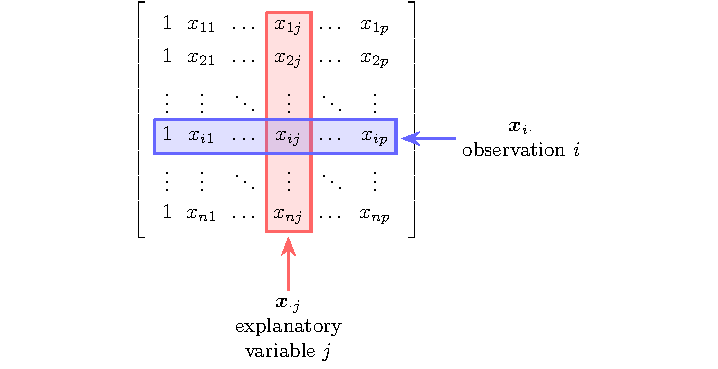
\includegraphics{_main_files/figure-latex/design-matrix-1} 

}

\caption{Design Matrix $\boldsymbol{X}$.}\label{fig:design-matrix}
\end{figure}

We can then express the GLM structural assumptions in a matrix form as:
\[
\boldsymbol{g}(\boldsymbol{\mu}) = \boldsymbol{X} \boldsymbol{\beta}
\]
where \(\boldsymbol{g}(\cdot)\) must be intended as the vectorial function that links every \(\mu_i\) to \(g(\mu_i)\).
\[
\begin{array}{cccc}
\boldsymbol{g}: & \mathbb{R}^n & \longrightarrow & \mathbb{R}^n \\
                & \left(
                    \begin{matrix} \mu_1  \\ \vdots \\ \mu_n \end{matrix}
                  \right)
                  & \longmapsto & 
                  \left(
                    \begin{matrix} g(\mu_1)  \\ \vdots \\ g(\mu_n) \end{matrix}
                  \right)
\end{array}
\]

We assume the design matrix to be a full rank matrix, i.e.~\(\text{rank}(\boldsymbol{X}) = p+1\). This assumption corresponds to assuming that \(\boldsymbol{X}\) columns are linearly independent.

The function \(g(\cdot)\) can be chosen as any monotonic function with continuous first and second derivatives. Given a family \(\mathcal{F}\), a common choice is its canonical link function that is defined as:
\[
g(\mu) = b'^{-1}(\mu)
\]
From \eqref{eq:exp-fam-expected-value} we we obtains that, as \(\mu = b'(\theta)\), choosing the canonical function corresponds to using \(\theta\) as the linear predictor:
\[
\eta = g(\mu) = b'^{-1}(\mu) = \theta
\]

In table \ref{tab:can-link-fun} the canonical link functions for the families mentioned in \ref{tab:exp-families} are reported.

\begin{table}[!h]

\caption{\label{tab:can-link-fun}Canonical link functions.}
\centering
\begin{tabular}[t]{lccc}
\toprule
\textbf{Distribution} & \textbf{\makecell[c]{Cumulant function\\$b(\theta)$}} & \textbf{\makecell[c]{Derivative\\$b'(\theta)$}} & \textbf{\makecell[c]{Canonical link function\\$g(\mu)=b'^{-1}(\mu)$}}\\
\toprule\addlinespace
Normal & $\frac{\theta^2}{2}$ & $\theta$ & $\mu$\\
\addlinespace\hline\addlinespace
Poisson & $e^{\theta}$ & $e^\theta$ & $\log{(\mu)}$\\
\addlinespace\hline\addlinespace
Gamma & $-\log{\left(-\theta\right)}$ & $-\frac{1}{\theta}$ & $-\frac{1}{\mu}$\\
\addlinespace\hline\addlinespace
\makecell[l]{Scaled\\Binomial} & $\log\left(1+e^{\theta}\right)$ & $\frac{e^{\theta}}{1 + e^{\theta}}$ & $\log{\left( \frac{p}{1-p} \right)}$\\
\bottomrule
\end{tabular}
\end{table}

In Gamma case, its canonical function \(g(\mu)=-\frac{1}{\mu}\) has the drawback that it links the expected values \(\mu\in]0,+\infty[\) to \(\eta\in]-\infty, 0[\). This would require some constraints on \(\boldsymbol{\beta}\) because \(\eta=\boldsymbol{x}^t\boldsymbol{\beta}\) would have to be \(<0\). For this reason, it is preferred to use \(g(\mu) = \log(\mu)\) that maps \(]0, +\infty[\) to \(\mathbb{R}\).

In Scaled Binomial case the canonical function \(g(p) = \log{\left(\frac{p}{1-p}\right)}\) is called logit and its inverse \(g^{-1}(\eta) = \frac{e^{\eta}}{1 + e^{\eta}}\) is called logistic. For Scaled Binomial distribution we keep using the notation \(p\) for the expected value as it corresponds to the probability of success \(p\).

\hypertarget{model-fitting}{%
\subsubsection{Model fitting}\label{model-fitting}}

The model depends on the parameters \(\left(\boldsymbol{\beta}, \phi\right)\). Indeed, the parameters \(\theta_i\) can be obtained by \(\boldsymbol{\beta}\) as:
\[
\theta_i = b'^{-1}(\mu_i) = b'^{-1}(g^{-1}(\eta_i)) = b'^{-1}\left(g^{-1}\left(\boldsymbol{x}_i^t\boldsymbol{\beta}\right)\right)
\]

Therefore, fitting the model corresponds to estimating \(\left(\boldsymbol{\beta}, \phi\right)\). The technique used in GLM is the \emph{maximum likelihood}. Let's indicate with \(L\left(\boldsymbol{\beta}, \phi; \boldsymbol{y}\right)\) the model likelihood. We remind that the likelihood is a function of the parameters that maps \(\left(\boldsymbol{\beta}, \phi\right)\) to the density (or probability in the discrete case) of the observed values \(\boldsymbol{y}\) conditioned to the parameters \(\left(\boldsymbol{\beta}, \phi\right)\)
\[
\begin{array}{cccc}
L: & \mathbb{R}^{p+1} \times \Lambda & \longrightarrow & [0, +\infty[ \\
   & \left(\boldsymbol{\beta}, \phi\right) & \longmapsto & f_{\boldsymbol{Y}}(\boldsymbol{y}; \boldsymbol{\theta}, \phi)
\end{array}
\]

The maximum likelihood estimates are the values \(\left(\boldsymbol{\beta}, \phi\right)\) that maximize \(L\left(\boldsymbol{\beta}, \phi; \boldsymbol{y}\right)\). In practice, \(\boldsymbol{\beta}\) are the parameters of interest, while \(\phi\) is considered as a disturbance parameter. It is possible to show that conditioned to any \(\phi\), the value for \(\boldsymbol{\beta}\) that maximizes \(L(\cdot, \cdot)\) does not depend on \(\phi\). Therefore, \(\boldsymbol{\beta}\) and \(\phi\) can be estimated separately.

Let's indicate with \(\tilde{\boldsymbol{\beta}}\) the maximum likelihood estimator for \(\boldsymbol{\beta}\). Its determination \(\hat{\boldsymbol{\beta}}\) is defined as:

\begin{equation}
\label{eq:max-lik-est}
\hat{\boldsymbol{\beta}} = \argmax_{\boldsymbol{\beta}\in\mathbb{R}^{p+1}}{L\left(\boldsymbol{\beta}, \phi; \boldsymbol{y}\right)}
\end{equation}

Finding the values \(\hat{\boldsymbol{\beta}}\) that maximize the likelihood corresponds to finding the values that maximize the log-likelihood \(l\left(\boldsymbol{\beta}, \phi; \boldsymbol{y}\right) = \log{\left(L\left(\boldsymbol{\beta}, \phi; \boldsymbol{y}\right)\right)}\). For the independence hypothesis on \(Y_1, \dots, Y_n\) we get:

\begin{align}
\nonumber
l\left(\boldsymbol{\beta}, \phi; \boldsymbol{y}\right) & =
\log{\left(L\left(\boldsymbol{\beta}, \phi; \boldsymbol{y}\right)\right)}
\\ \nonumber & =
\log{\left(\prod_{i=1}^{n}{\exp{\left\{ \frac{\omega_i}{\phi} \left[y_i\theta_i - b(\theta_i) \right] \right\}} c(y_i, \phi, \omega_i)}\right)}
\\ \label{eq:log-like} & =
\sum_{i=1}^{n}{
\left\{
\frac{\omega_i}{\phi} \left[y_i\theta_i - b(\theta_i) \right] + \log{\left(c(y_i, \phi, \omega_i)\right)}
\right\}
}
\\ \nonumber & =
\sum_{i=1}^{n}{l_i\left(\boldsymbol{\beta}, \phi; \boldsymbol{y}\right)}
\end{align}

The maximum value of \(l\left(\boldsymbol{\beta}, \phi; \boldsymbol{y}\right)\) can be obtained by imposing all its partial derivatives equal to \(0\):
\[
\frac{\partial l\left(\boldsymbol{\beta}, \phi; \boldsymbol{y}\right)}
{\partial\beta_j}
= 0, \quad \forall j\in\{0,1,\dots,p\}
\]

These equations can be solved with numerical methods, such as Newton-Raphson algorithm or its variant Fisher scoring. It is possible to show that Newton-Raphson algorithm corresponds to iteratively solving a weighted least squares optimization problem.

A statistic that can be used to measures the goodness of fit of a model is the \emph{Deviance}. It can be used by comparing the current model log-likelihood \(l\left(\hat{\boldsymbol{\beta}}, \phi; \boldsymbol{y}\right)\) with the \emph{saturated model} log-likelihood \(l_{S}\left(\boldsymbol{\beta}^*, \phi; \boldsymbol{y}\right)\). The saturated model is the model with \(n\) parameter, so a model where the expected values of the response variables \(\mu_1, \dots, \mu_n\) are estimated with their observed values \(y_1, \dots, y_n\). It is possible to show that \(l_{S}\left(\boldsymbol{\beta}^*, \phi; \boldsymbol{y}\right) \ge l\left(\hat{\boldsymbol{\beta}}, \phi; \boldsymbol{y}\right)\). The closer \(l\left(\hat{\boldsymbol{\beta}}, \phi; \boldsymbol{y}\right)\) is to \(l_{S}\left(\boldsymbol{\beta}^*, \phi; \boldsymbol{y}\right)\), the better the current model fitting is.

\begin{definition}[Deviance]
\label{def:deviance-def} \iffalse (Deviance) \fi{} Given \(l\left(\hat{\boldsymbol{\beta}}, \phi; \boldsymbol{y}\right)\) the log-likelihood of the current model and \(l_{S}\left(\boldsymbol{\beta}^*, \phi; \boldsymbol{y}\right)\) the log-likelihood of the saturated model, the \textit{Scaled Deviance} of the current model is defined as:
\[
S(\hat{\boldsymbol{\beta}}, \phi, \boldsymbol{y}) =
-2\left(
l\left(\hat{\boldsymbol{\beta}}, \phi; \boldsymbol{y}\right)
- l_{S}\left(\boldsymbol{\beta}^*, \phi; \boldsymbol{y}\right)
\right)
\]
The \textit{Deviance} of the current model is defined as:
\[
D(\hat{\boldsymbol{\beta}}, \boldsymbol{y}) =
\phi \, S(\hat{\boldsymbol{\beta}}, \phi, \boldsymbol{y})
\]
\end{definition}

In deviance notation \(D(\hat{\boldsymbol{\beta}}, \boldsymbol{y})\), the parameter \(\phi\) is not reported because the deviance does not depend on \(\phi\). Indeed, from \eqref{eq:log-like} we get:

\begin{align*}
S(\hat{\boldsymbol{\beta}}, \phi, \boldsymbol{y})
& =
-2\left(
l\left(\hat{\boldsymbol{\beta}}, \phi; \boldsymbol{y}\right)
- l_{S}\left(\boldsymbol{\beta}^*, \phi; \boldsymbol{y}\right)
\right)
\\ & =
-2\left(
\sum_{i=1}^{n}{
\left\{
\frac{\omega_i}{\phi} \left[y_i\hat{\theta}_i - b(\hat{\theta}_i) \right] + \log{\left(c(y_i, \phi, \omega_i)\right)}
\right\}
}
\right.
\\ & \qquad \qquad -
\left.
\sum_{i=1}^{n}{
\left\{
\frac{\omega_i}{\phi} \left[y_i\theta_i^* - b(\theta_i^*) \right] + \log{\left(c(y_i, \phi, \omega_i)\right)}
\right\}
}
\right)
\\ & =
-2\left(
\sum_{i=1}^{n}{
\frac{\omega_i}{\phi}
\left\{
\left[y_i\hat{\theta}_i - b(\hat{\theta}_i) \right]
- \left[y_i\theta_i^* - b(\theta_i^*) \right]
\right\}
}
\right)
%
\\[12pt]
%
D(\hat{\boldsymbol{\beta}}, \boldsymbol{y})
& =
-2\left(
\sum_{i=1}^{n}{
\omega_i
\left\{
\left[y_i\hat{\theta}_i - b(\hat{\theta}_i) \right]
- \left[y_i\theta_i^* - b(\theta_i^*) \right]
\right\}
}
\right)
\end{align*}

In table \ref{tab:deviance} the deviances for the families mentioned in \ref{tab:exp-families} are reported.

\begin{table}[!h]

\caption{\label{tab:deviance}Deviance for Linear Exponential Families}
\centering
\begin{tabular}[t]{lc}
\toprule
\textbf{Distribution} & \textbf{Deviance $D(\hat{\boldsymbol{\beta}}, \boldsymbol{y})$}\\
\toprule\addlinespace
Normal & $\sum_{i=1}^{n}{\left( y_i - \hat{\mu}_i \right)^2}$\\
\addlinespace\hline\addlinespace
Poisson & $2\,\sum_{i=1}^{n}{\left\{ y_i \log{\left(\frac{y_i}{\hat{\mu}_i}\right)} - \left( y_i - \hat{\mu}_i \right) \right\}}$\\
\addlinespace\hline\addlinespace
Gamma & $2\,\sum_{i=1}^{n}{\left\{ - \log{\left(\frac{y_i}{\hat{\mu}_i}\right)} + \frac{ y_i - \hat{\mu}_i }{\hat{\mu}_i} \right\}}$\\
\addlinespace\hline\addlinespace
\makecell[l]{Scaled\\Binomial} & $2\,\sum_{i=1}^{n}{\left\{ y_i \log{\left(\frac{y_i}{\hat{\mu}_i}\right)}+ \left(1-y_i\right) \log{\left(\frac{1-y_i}{1-\hat{\mu}_i}\right)} \right\}}$\\
\bottomrule
\end{tabular}
\end{table}

As \(l_{S}\left(\boldsymbol{\beta}^*, \phi; \boldsymbol{y}\right)\) does not depend on \(\hat{\boldsymbol{\beta}}\), maximizing the likelihood in equation \eqref{eq:max-lik-est} is the same as minimizing the deviance, that can be seen as a \emph{Loss Function}.

\hypertarget{variable-effects}{%
\subsubsection{Variable effects}\label{variable-effects}}

As we mentioned in \ref{chap:pricing-variables-encoding}, the explanatory variables can be \emph{quantitative} or \emph{qualitative}. In GLM, if explanatory variables transformation terms aren't added to the linear predictor \(\eta\), the variables effect on \(\eta\) is linear. In figure \ref{fig:expl-var-types} the effects of quantitative and qualitative variables are shown. The data is simulated from a GLM with Normal response and identity link.





\begin{figure}[!hbtp]

{\centering \subfloat[Quantitative\label{fig:expl-var-types-1}]{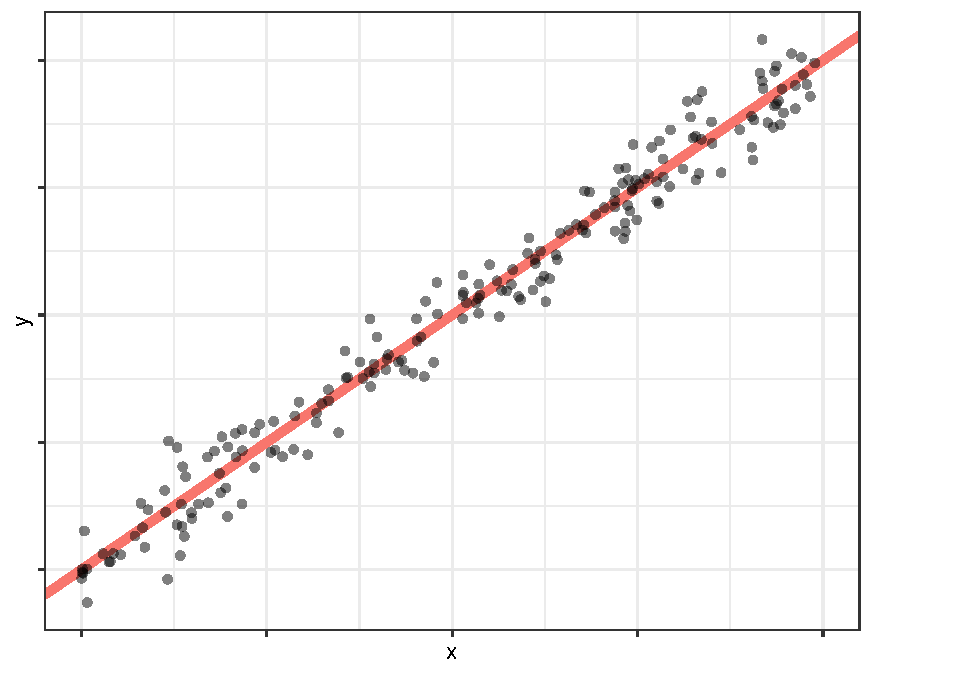
\includegraphics[width=0.5\linewidth]{_main_files/figure-latex/expl-var-types-1} }\subfloat[Qualitative\label{fig:expl-var-types-2}]{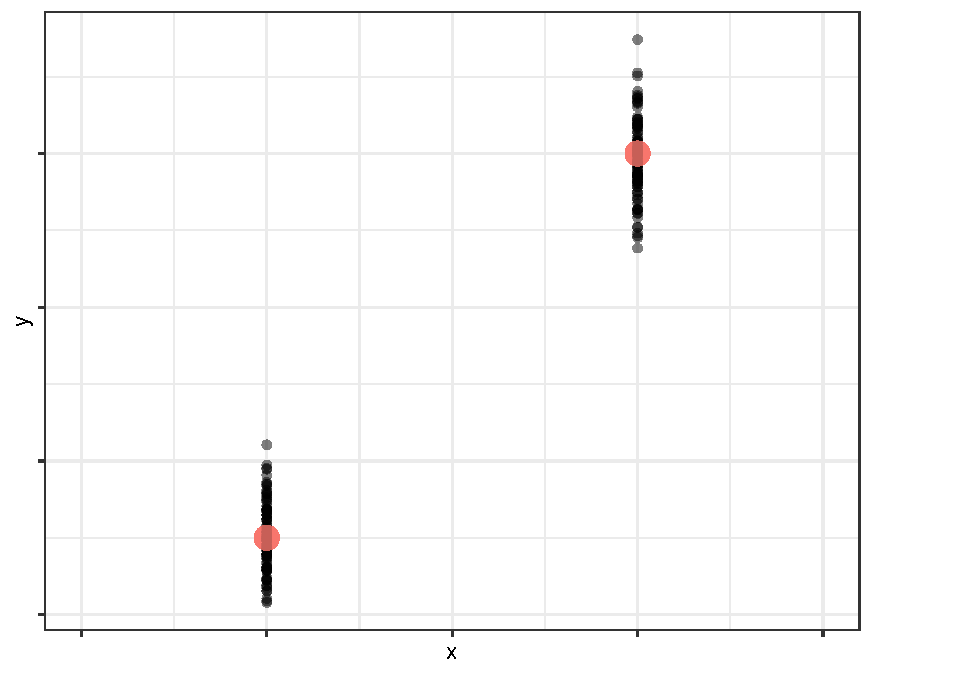
\includegraphics[width=0.5\linewidth]{_main_files/figure-latex/expl-var-types-2} }\newline\subfloat[Quantitative and qualitative \\ without interaction\label{fig:expl-var-types-3}]{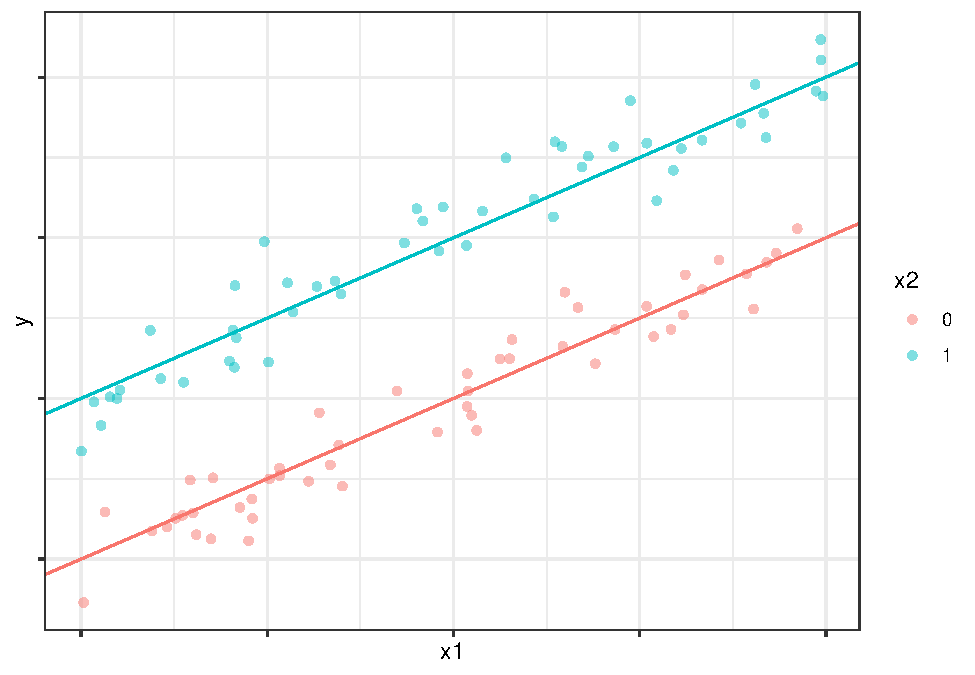
\includegraphics[width=0.5\linewidth]{_main_files/figure-latex/expl-var-types-3} }\subfloat[Quantitative and qualitative \\ with interaction\label{fig:expl-var-types-4}]{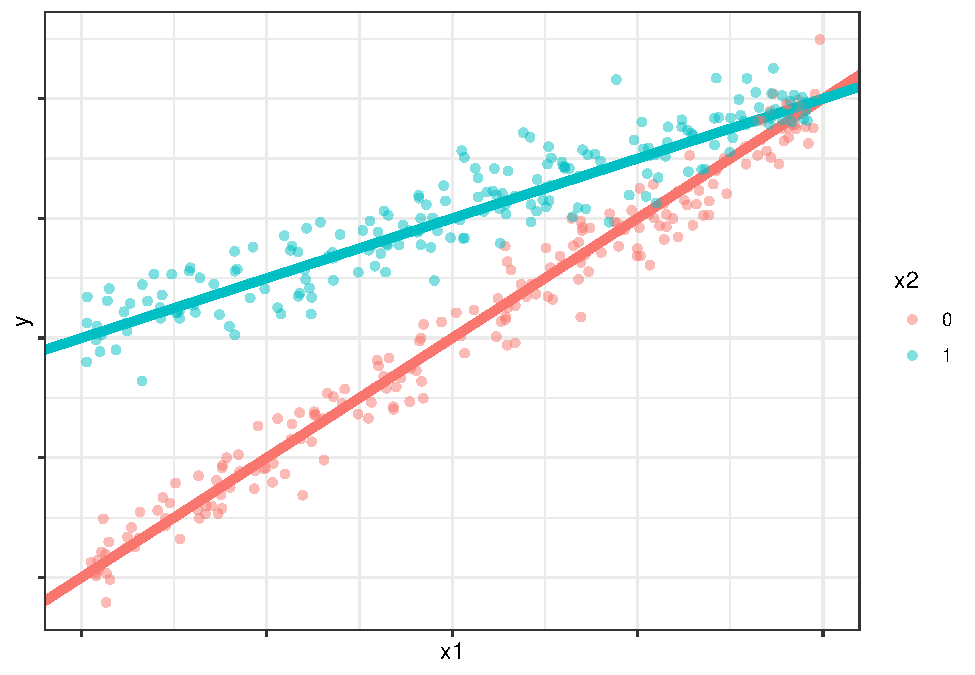
\includegraphics[width=0.5\linewidth]{_main_files/figure-latex/expl-var-types-4} }

}

\caption{Explanatory variables types.}\label{fig:expl-var-types}
\end{figure}

In top-left panel, we see the effect of the quantitative variable \(x\) in the model \(\mu_i = \beta_0 + \beta_1 x_i\). As we can see it is a straight line. The coefficient \(\beta_1\) represents the slope of the line, thus \(\beta_1>0\) means that \(x\) and \(Y\) are positively correlated, while \(\beta_1<0\) means that \(x\) and \(Y\) are negatively correlated. For example, if \(x\) is the power of the vehicle and \(Y\) the yearly number of claims, \(\beta_1>0\) means that the more powerful the vehicle is, the more claims the policyholder will experience on average.

In top-right panel, we see the effect of a qualitative binary variable \(x\) in the model \(\mu_i = \beta_0 + \beta_1 x_i\). The variable is encoded with values \(0\) and \(1\), so \(\beta_1\) represents the effect of the modality \(x=1\). In general, for a qualitative variable with \(K\) modalities we will have \(K-1\) dummy variables \(x'_1, \dots, x'_{K-1}\) and the model will be \(\mu_i = \beta_0 + \beta_1 x'_{i1} + \beta_2 x'_{i2} + \dots + + \beta_{K-1} x'_{i, K-1}\). Thus, the \(\beta_j\) coefficient represents the relative effect of the modality \(j\) compared to the base level modality, that is the one not explicitly included in the dummy encoding. For example, if \(x\) is the vehicle make, \(Y\) the yearly number of claims, the base level for \(x\) is `Fiat' and the \(j\)\textsuperscript{th} modality is `Ferrari', then \(\beta_j>0\) means that Ferrari cars on average experience more claims that Fiat cars.

In general, in a multivariate model, the coefficient \(\beta_j\) represents the effect of the variable \(j\) given all the others. For example, in the example of Fiat and Ferrari cars, if in the model there is also the variable `vehicle power', the coefficient \(\beta_j\) corresponding to the modality `Ferrari' represents the how more risky a Ferrari car is compared to a Fiat car with the same power. If the explanatory variables are strongly correlated, it is important to be aware of this aspect. For example, Ferrari cars are usually more powerful that Fiat cars. So, it is possible that in general Ferrari cars are more risky than Fiat cars, but comparing a Ferrari car to a Fiat with the same power, the Ferrari could be less risky. This effect is called \emph{Simpson's paradox} \footnote{\url{https://en.wikipedia.org/wiki/Simpson\%27s_paradox}}.

In bottom-left panel of figure \ref{fig:expl-var-types}, we see the effect of a quantitative variable \(x_1\) and a qualitative binary variable \(x_2\) together in the model \(\mu_i = \beta_0 + \beta_1 x_{i1} + \beta_2 x_{i2}\). As we can seen, the effects of \(x_1\) variable in the two groups defined by \(x_2\) variable are represented by two parallel straight lines. The first one is \(\mu_i = \beta_0 + \beta_1 x_{i1}\) and the second is \(\mu_i = \left(\beta_0 + \beta_2\right) + \beta_1 x_{i1}\). The coefficient \(\beta_2\) represents the vertical distance between the two lines.

In bottom-right panel, the interaction effect between \(x_1\) and \(x_2\) is included in the model. The model becomes \(\mu_i = \beta_0 + \beta_1 x_{i1} + \beta_2 x_{i2} + \beta_3 x_{i1} x_{i2}\). That means that the effect of \(x_1\) variables depends on the determination of the \(x_2\) variable. In the group with \(x_2=0\) the effect is represented by the line \(\mu_i = \beta_0 + \beta_1 x_i\); the group with \(x_2=1\) the effect is represented by the line \(\mu_i = \left(\beta_0 + \beta_2\right) + \left(\beta_1 + \beta_3\right) x_{i1}\).

For quantitative variables, it is possible to consider also non linear effects in GLMs. Some examples are reported in figure \ref{fig:expl-var-quant-effect}.





\begin{figure}[!hbtp]

{\centering \subfloat[Polynomial degree 2\label{fig:expl-var-quant-effect-1}]{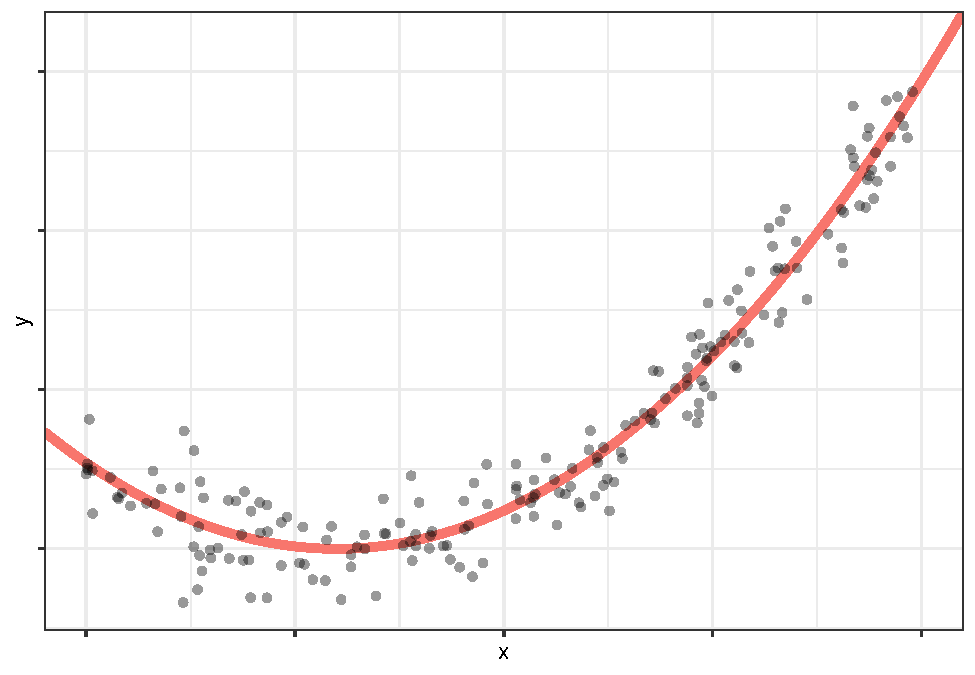
\includegraphics[width=0.5\linewidth]{_main_files/figure-latex/expl-var-quant-effect-1} }\subfloat[Polynomial degree 4\label{fig:expl-var-quant-effect-2}]{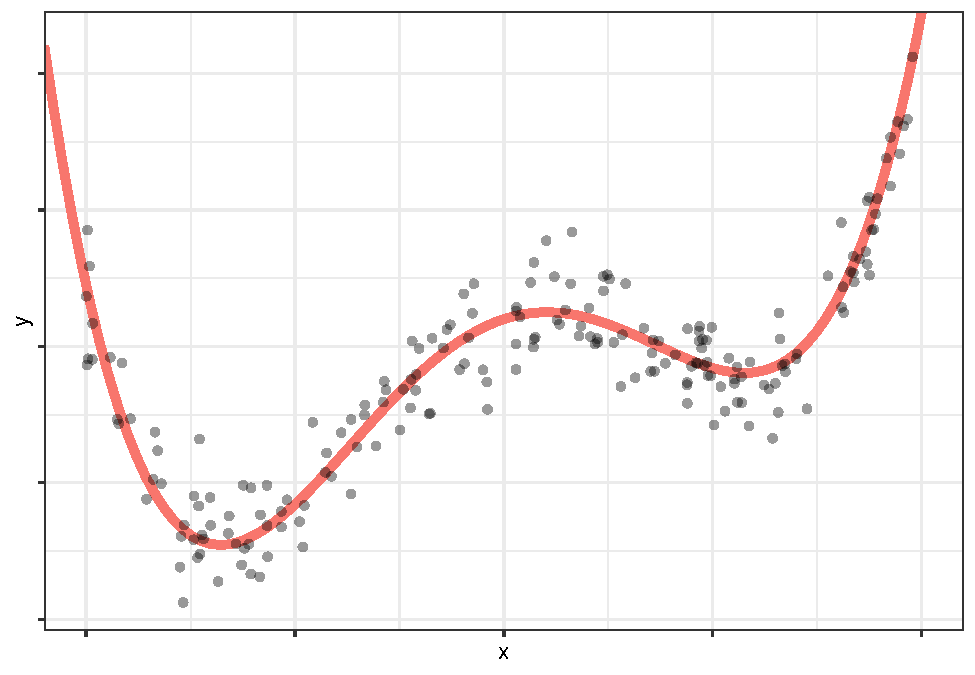
\includegraphics[width=0.5\linewidth]{_main_files/figure-latex/expl-var-quant-effect-2} }\newline\subfloat[Piece-wise linear\label{fig:expl-var-quant-effect-3}]{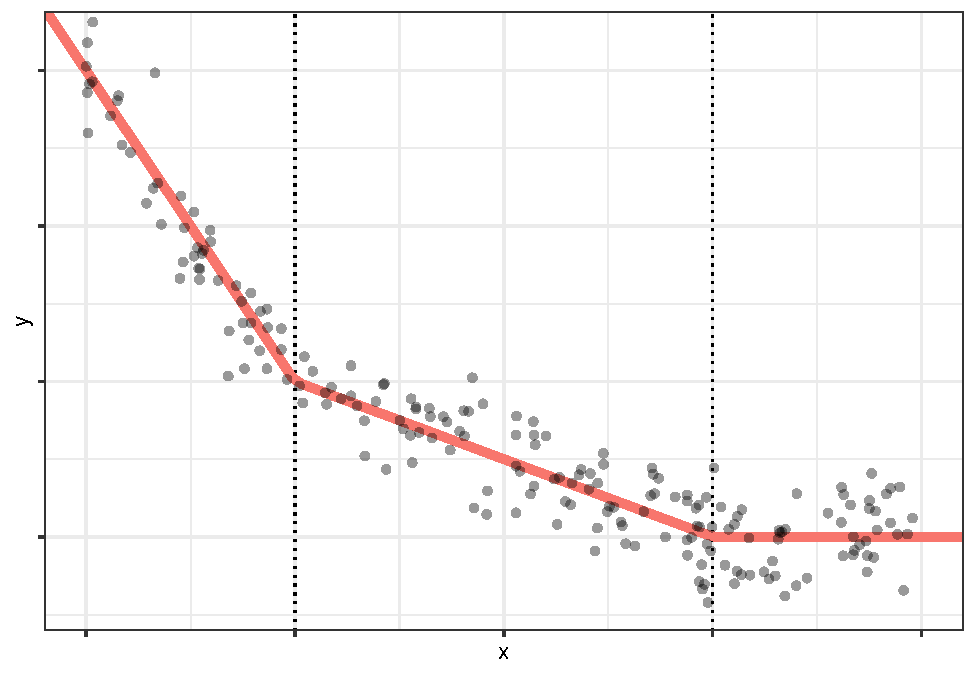
\includegraphics[width=0.5\linewidth]{_main_files/figure-latex/expl-var-quant-effect-3} }\subfloat[Piece-wise polynomial degree 2\label{fig:expl-var-quant-effect-4}]{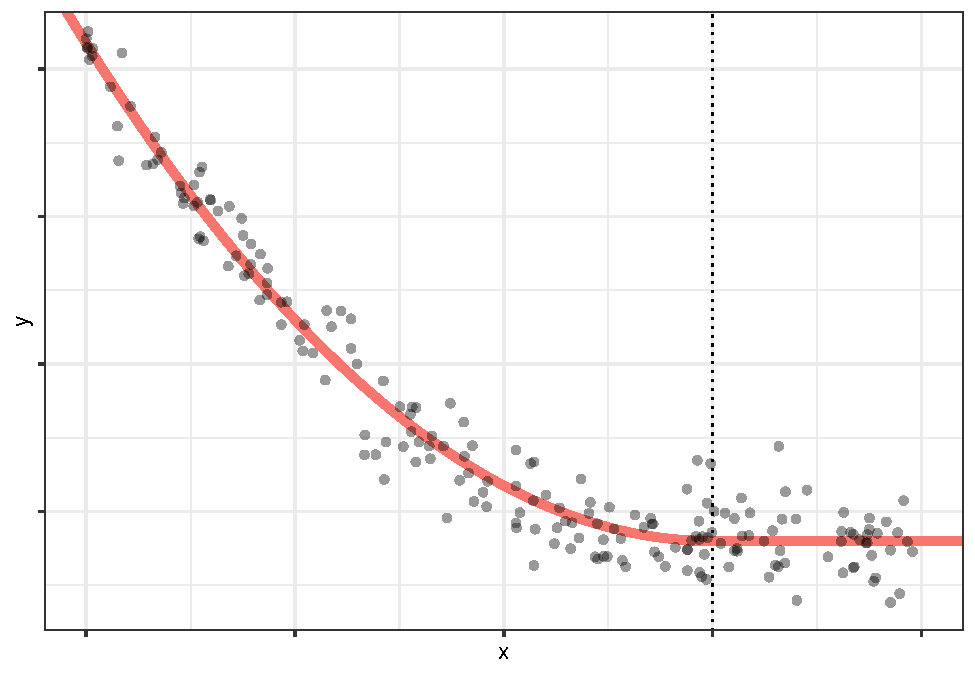
\includegraphics[width=0.5\linewidth]{_main_files/figure-latex/expl-var-quant-effect-4} }

}

\caption{Explanatory quantitative variables effects.}\label{fig:expl-var-quant-effect}
\end{figure}

The basic way to achieve it is by adding polynomial terms to the linear predictor. For instance, if \(x\) is a quantitative variable, it is possible to add to the model the term \(x^2\), obtaining the model \(\mu_i = \beta_0 + \beta_1 x_{i} + \beta_2 x_i^2\). An example of model with both \(x\) and \(x^2\) terms is represented in top-left panel of figure \ref{fig:expl-var-quant-effect}. Adding the quadratic term, the effect graph becomes a parabola.

With the same logic, it is possible to add more power terms. In general, if we want to model \(x\) with a polynomial of degree \(d\), we can consider the model \(\mu_i = \beta_0 + \beta_1 x_{i} + \beta_2 x_{i}^2 + \dots + \beta_d x_{i}^d\). In top-right panel of figure \ref{fig:expl-var-quant-effect} a 4\textsuperscript{th} degree polynomial effect is represented. We highlight that the model is still considered linear, as the attribute ``Linear'' in ``General Linear Model'' is referred to the relation between the parameters \(\beta_j\) and the linear predictor \(\eta_i\) that is still linear.

Another way to model non liner effects of explanatory variables is to separate the effects by pieces. In bottom-left panel of figure \ref{fig:expl-var-quant-effect} a case in which the \(x\) effect is separated in 3 pieces is represented. As in all the pieces the effect is linear, the graph of the variable effect is a broken line. This effect can be achieved by adding to the model the terms \((x-\nu)_+\), where \((x)_+\) represents the positive part of \(x\) (\((x)_+ = \max(0,x)\)) and \(\nu\) is the value of \(x\) in the angular point. The \(\nu\) values are called \emph{nodes}, If the nodes are \(\nu_1, \nu_2, \dots, \nu_m\), the model can be represented as \(\mu_i = \beta_0 + \beta_1 x_i + \beta_2 (x_i-\nu_1)_+ + \beta_3 (x_i-\nu_2)_+ + \dots + \beta_{m+1} (x_i-\nu_m)_+\). This kind of functions are called \emph{linear splines} and will be further discussed in section \ref{chap:gam}. If we want the effect to be null from a certain point \(\nu\), we can consider the variable \(x' = \min(\nu, x)\) instead of \(x\). This corresponds to aggregate to \(\nu\) all the \(x\) after \(\nu\).

The piece-wise approach can be enhanced by also considering polynomial terms. For instance, in bottom-left panel of figure \ref{fig:expl-var-quant-effect}, the model represented is \(\mu_i = \beta_0 + \left( x_i - \nu \right)_-^2\), where \((x)_-\) is the negative part of \(x\) (\((x)_- = \min(0,x)\)). \(f(x) = (x-\nu)^2\) is a parabola with vertex in \(\nu\). The fact of not adding the linear term leads to a monotonic effect made by a semi-parabola and a horizontal semi-line that starts from its vertex.

The examples represented in figures \ref{fig:expl-var-types} and \ref{fig:expl-var-quant-effect} are based on simulated data. That means that the linear predictor structure is known and the coefficients \(\beta_0, \beta_1, \dots, \beta_J\) are known. In practice, the real model is not known and the coefficients and the structure must be estimated by the data. Thus, we can take assumptions on the structure and we can estimate the coefficients with \(\hat{\beta}_0, \hat{\beta}_1, \dots, \hat{\beta}_J\). In many cases it is not so clear whether to consider or not a variable and how to consider it. For example, with the same data both bottom-left and bottom-right models could work fine. In section \ref{chap:variable-selection} we are going to discuss some variable selection techniques for GLM.

\hypertarget{link-functions-and-relativities}{%
\subsubsection{Link functions and relativities}\label{link-functions-and-relativities}}

As we mentioned in \ref{chap:linear-exp-families}, GLM supports several families. In figure \ref{fig:resp-var} the models \(g(\mu_i) = \beta_0 + \beta_1 x_i\) with different response variable distributions and link functions are represented. As we can see from the plots, a linear effect on \(x\) corresponds to a logistic effect when the link is logit and to an exponential effect when the link is log.





\begin{figure}[!hbtp]

{\centering \subfloat[Normal - identity\label{fig:resp-var-1}]{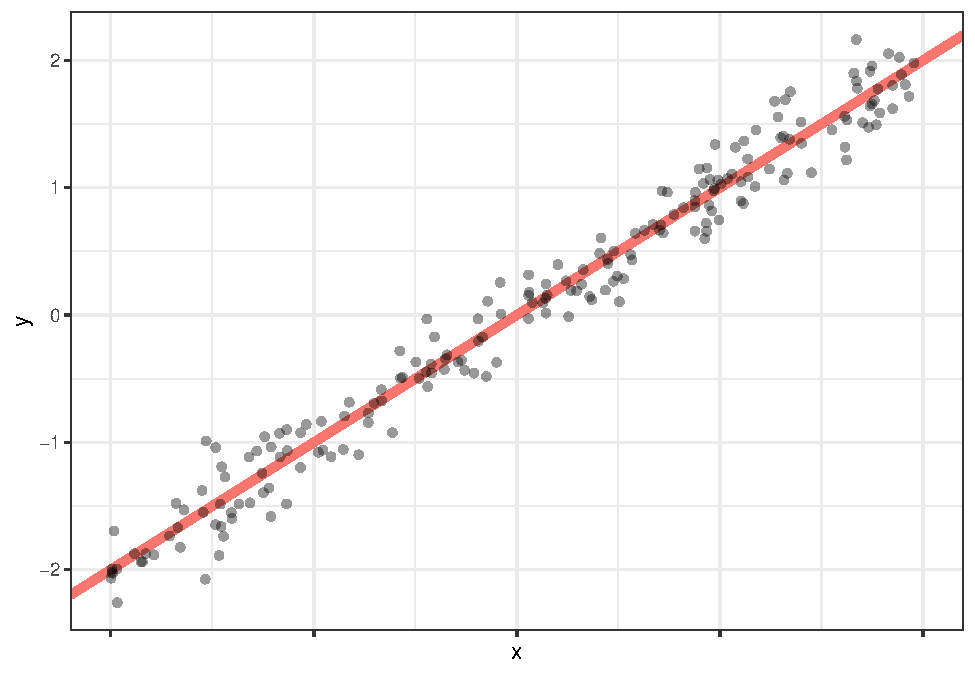
\includegraphics[width=0.5\linewidth]{_main_files/figure-latex/resp-var-1} }\subfloat[Binomial - logit\label{fig:resp-var-2}]{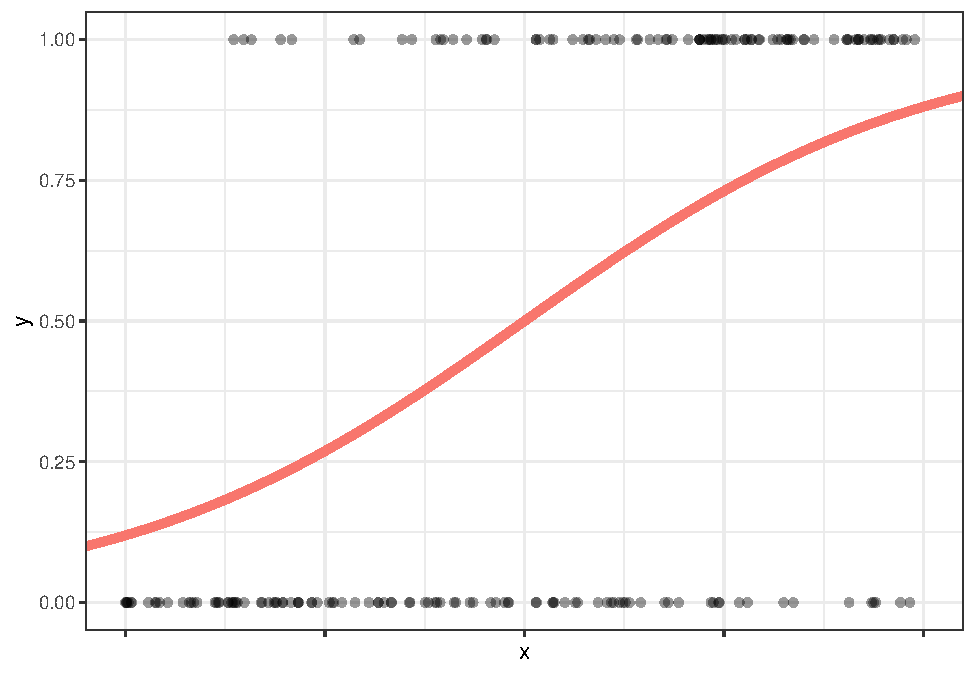
\includegraphics[width=0.5\linewidth]{_main_files/figure-latex/resp-var-2} }\newline\subfloat[Poisson - log\label{fig:resp-var-3}]{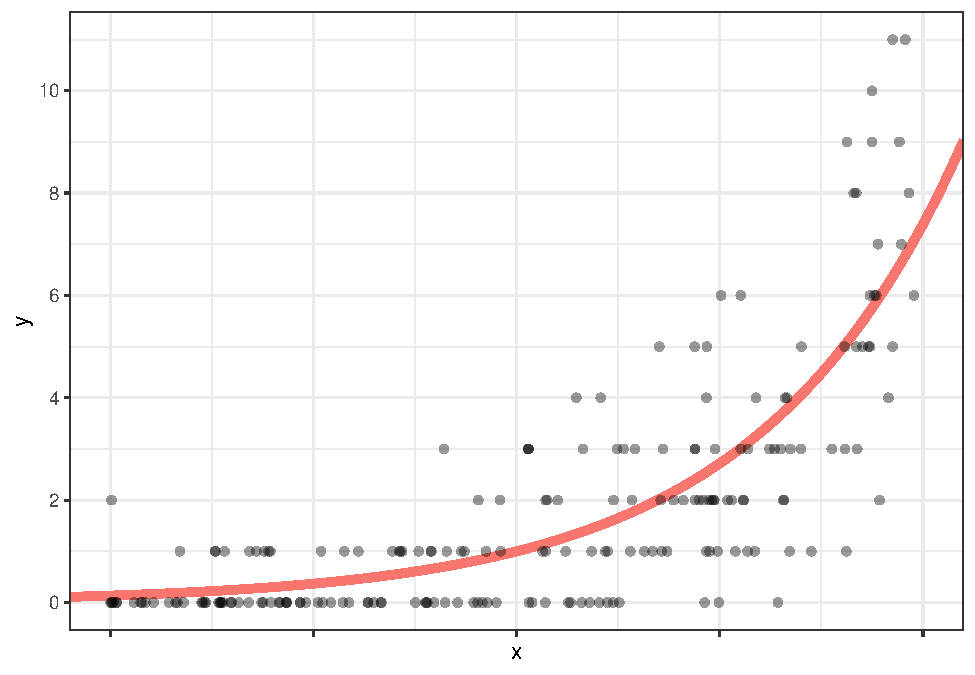
\includegraphics[width=0.5\linewidth]{_main_files/figure-latex/resp-var-3} }\subfloat[Gamma - log\label{fig:resp-var-4}]{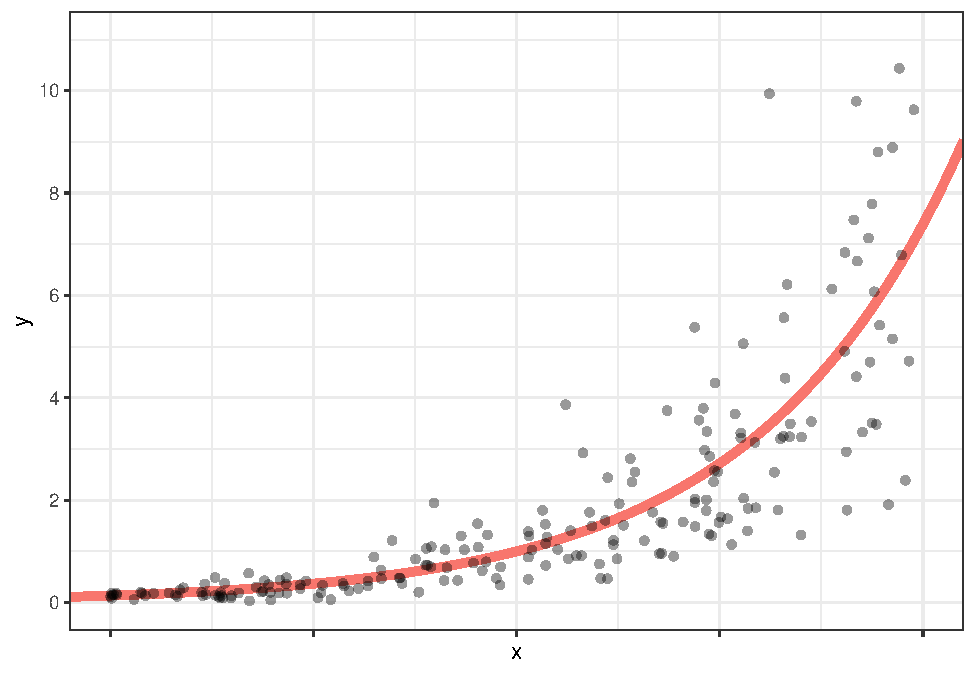
\includegraphics[width=0.5\linewidth]{_main_files/figure-latex/resp-var-4} }

}

\caption{Response variables and link functions.}\label{fig:resp-var}
\end{figure}

If \(g(\mu) = \log(\mu)\), the model structure can be expressed as:

\begin{align*}
\mu_i & = e^{\beta_0 + \beta_1 x_{i1} + \beta_2 x_{i2} + \dots + \beta_p x_{ip}} \\
& = e^{\beta_0} \left(e^{\beta_1}\right)^{x_{i1}} \left(e^{\beta_2}\right)^{x_{i2}} \dots \left(e^{\beta_p}\right)^{x_{ip}}
\end{align*}

The term \(e^{\beta_j}\) can be seen as the multiplicative relativity corresponding to the variable \(x_j\). If \(x_j\) is a dummy variable, \(e^{\beta_j}\) is the factor the expected value \(\mu_i\) is multiplied by when \(x_{ij}=1\). If \(x_j\) is a quantitative variable, \(e^{\beta_j}\) is the factor the expected value \(\mu_i\) is multiplied by for every one-unit increasing of \(x_{ij}\). Indeed:
\[\left(e^{\beta_j}\right)^{x_j+1} = e^{\beta_j} \left(e^{\beta_j}\right)^{x_j}\]

The fact that with log link the relation between coefficients \(\beta_0, \beta_1, \dots, \beta_p\) and expected value \(\mu_i\) becomes multiplicative is particularly useful to deal with exposure \(v_i\). In section \ref{chap:exposure} we have seen that often the observations are couples (policy, accounting year), so they have different exposures \(v_i\). Thus, we usually work with the number of claims occurred in the exposure period \(M_i\) and we observe its realization \(m_i\). The assumption we take is that:
\[M_i \sim Poisson(v_i \mu_i)\]
where \(\mu_i\) is the expected value of the yearly number of claims \(N_i\).

Under the GLM assumptions, we obtain

\begin{align*}
E(M_i) & = v_i \mu_i = v_i e^{\beta_0 + \beta_1 x_{i1} + \dots + \beta_p x_{ip}} \\
& = e^{\log(v_i)}e^{\beta_0 + \beta_1 x_{i1} + \dots + \beta_p x_{ip}} \\
& = e^{\beta_0 + \beta_1 x_{i1} + \dots + \beta_p x_{ip} + \log(v_i)}
\end{align*}

That means that we can model \(M_1, M_2, \dots, M_n\) as response variables in a GLM with Poisson response in which the linear predictor depends on an offset additive term \(\log(v_i)\).

If \(g(p) = \text{logit}(p)\), the model structure can be expressed as:

\begin{align*}
\frac{p_i}{1-p_i} & = e^{\beta_0 + \beta_1 x_{i1} + \beta_2 x_{i2} + \dots + \beta_p x_{ip}} \\
& = e^{\beta_0} \left(e^{\beta_1}\right)^{x_{i1}} \left(e^{\beta_2}\right)^{x_{i2}} \dots \left(e^{\beta_p}\right)^{x_{ip}}
\end{align*}

Thus, the term \(e^{\beta_j}\) can be seen as the multiplicative relativity corresponding to the variable \(x_j\). However, in this case the relativity doesn't multiply directly the probability of success \(p\), but it multiplies the odds of success \(\frac{p}{1-p}\).

\hypertarget{chap:variable-selection}{%
\subsubsection{Variable selection}\label{chap:variable-selection}}

One of the most challenging aspects of GLM fitting is selecting the variables and their effects by looking to observed data. In practice we usually have many explanatory variables available but only some of them are relevant for the prediction of the response variable. Adding useless variables to the model increases the variance of the estimators of the coefficients \(\tilde{\beta}_0, \tilde{\beta}_1, \dots, \tilde{\beta}_p\) and then the variance of \(\tilde{\mu}_i = \tilde{\beta}_0 + \tilde{\beta}_1 x_{i1} + \dots + \tilde{\beta}_p x_{ip}\). On the other hand, being too frugal with explanatory variables could lead to waste part of the predictive power of the available explanatory variables.

One useful tool we have to understand if an explanatory variable \(x\) is relevant or not is plotting the points \((x_i, y_i)\), as we did in \ref{fig:expl-var-types}, \ref{fig:expl-var-quant-effect} and \ref{fig:resp-var}. If there are too many observations and the plot is not easily readable, it is possible to group the points by \(x\) modalities and show for each group the average of \(y_i\) and a confidence interval that gives an idea on the dispersion of the observations around the average. If \(x\) is a continuous variable with too many modalities, it is possible to group them into buckets. Showing the average of \(y_i\) for groups of \(x\) is particularly useful for Binomial and Poisson data, where the fact that \(y_i\) can present few different values compromises the plot readability. An example is reported in figure \ref{fig:var-selection}. The top-left and bottom-left panels represent a case in which \(x\) and \(y\) are not related, while the top-right and bottom-right panels represent a case of positive correlation. From the ungrouped plot in the top-right panel the effect is not clear, while from bottom-right panel it is evident.





\begin{figure}[!hbtp]

{\centering \subfloat[No effect - ungrouped\label{fig:var-selection-1}]{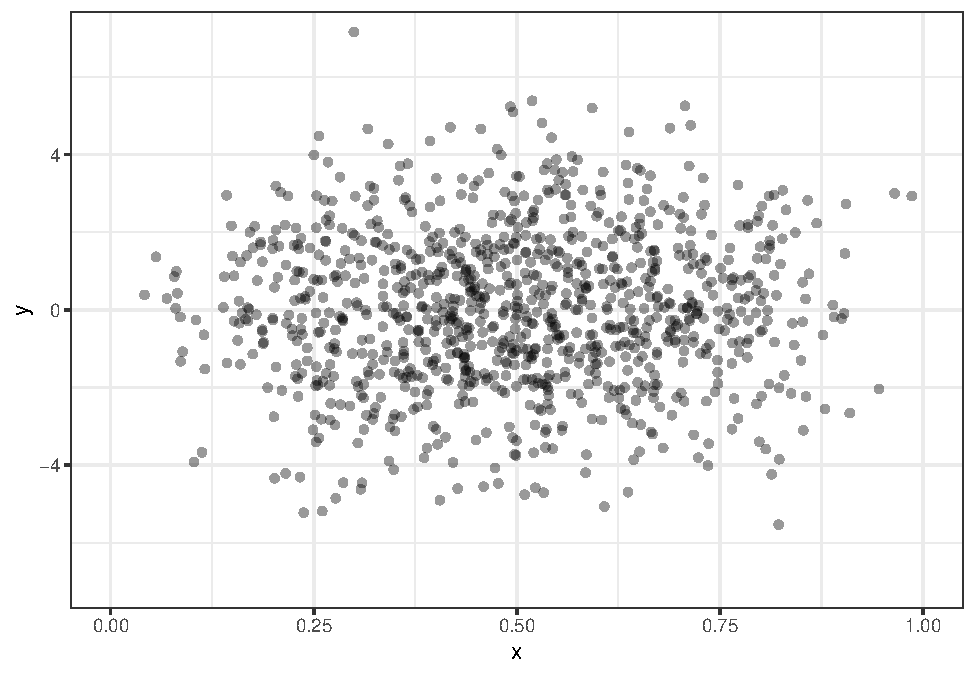
\includegraphics[width=0.5\linewidth]{_main_files/figure-latex/var-selection-1} }\subfloat[Positive effect - ungrouped\label{fig:var-selection-2}]{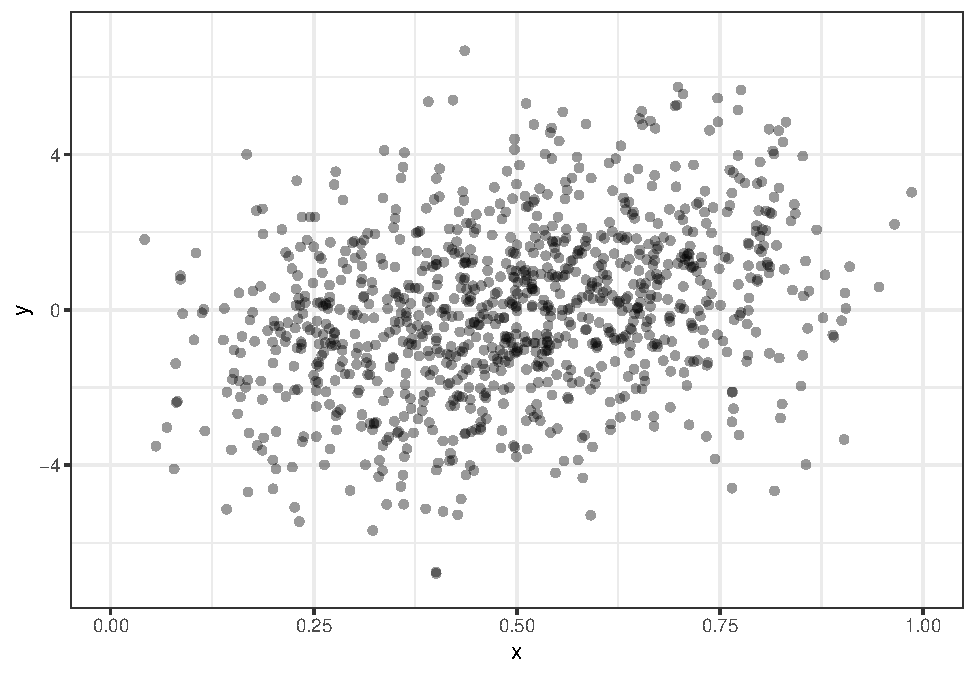
\includegraphics[width=0.5\linewidth]{_main_files/figure-latex/var-selection-2} }\newline\subfloat[No effect - grouped\label{fig:var-selection-3}]{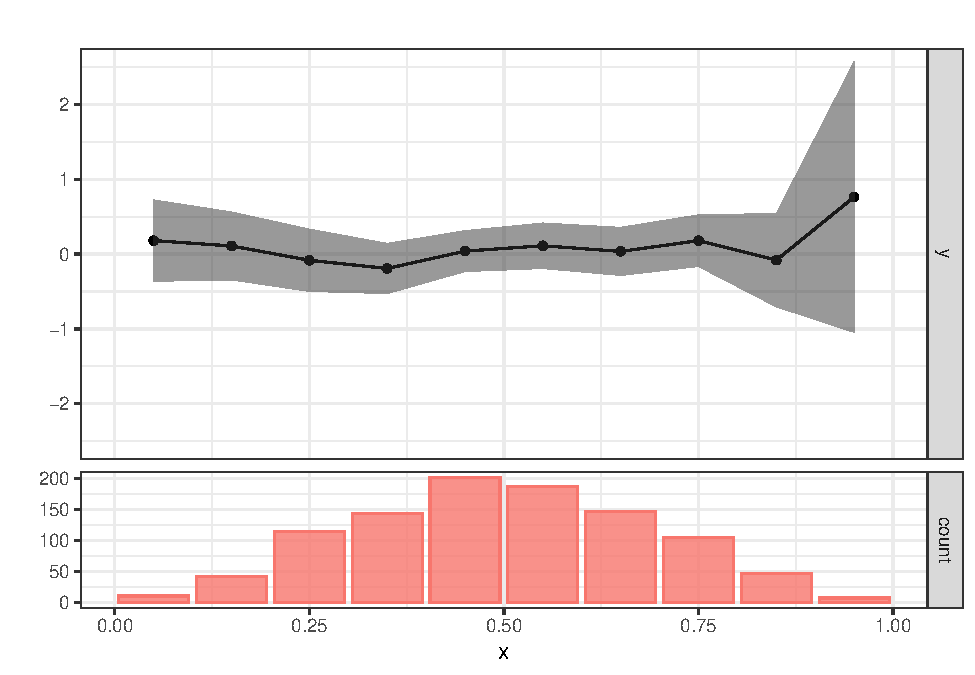
\includegraphics[width=0.5\linewidth]{_main_files/figure-latex/var-selection-3} }\subfloat[Positive effect - grouped\label{fig:var-selection-4}]{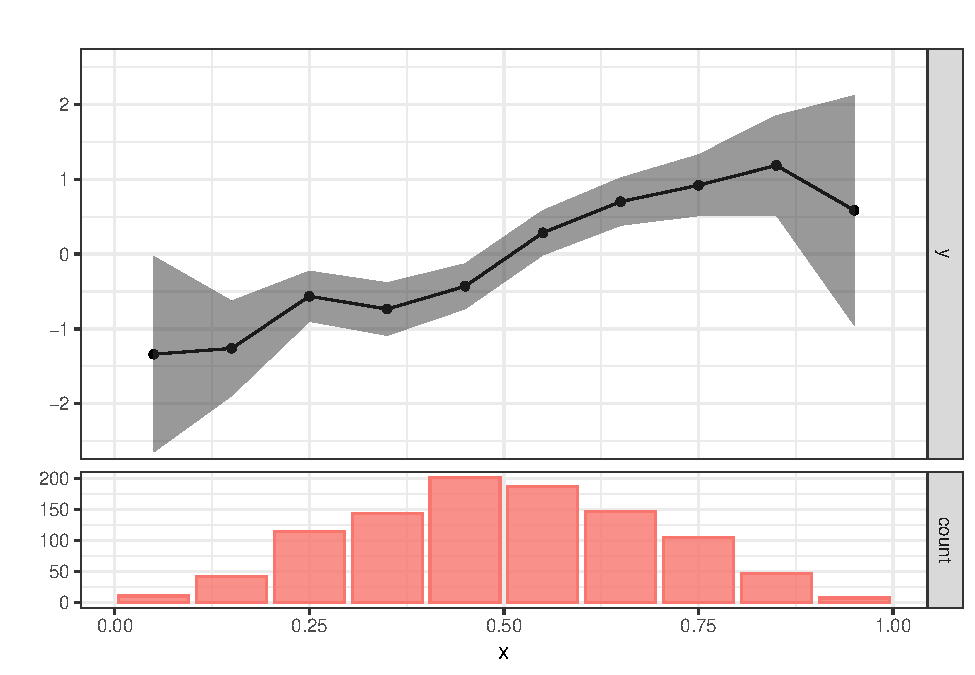
\includegraphics[width=0.5\linewidth]{_main_files/figure-latex/var-selection-4} }

}

\caption{Explanatory variable effect evaluation.}\label{fig:var-selection}
\end{figure}

If we are dealing with a multivariate model where we already inserted the variables \(x_1, \dots, x_p\) and we want to evaluate the additional information \(x_{p+1}\) brings, it is possible to look at the plot \((x_{i, p+1}, r_i)\), where \(r_i\) are the residuals of the model without the variable \(x_{p+1}\):
\[
r_i = y_i - \hat{\mu}_i = y_i - g^{-1}\left( \hat{\beta}_0 + \hat{\beta}_1 x_{i1} + \dots + \hat{\beta}_p x_{ip} \right)
\]

If the plot shows a clear trend, we will add the variable \(x\) to the model, otherwise we won't.

The choice of adding or not a variable in the model can be supported by \emph{hypothesis testing}.

\newpage

\hypertarget{elastic-net}{%
\subsection{Elastic Net}\label{elastic-net}}

Lorem ipsum dolor sit amet, consectetur adipiscing elit. Vivamus id mauris interdum, malesuada ante eu, tempus lacus. Aliquam blandit tortor a velit ultricies, eget pharetra nulla egestas. Suspendisse pellentesque finibus est, vitae ullamcorper magna convallis ut. Nulla a lectus in ligula iaculis convallis. Pellentesque tortor mauris, tempor nec dictum et, facilisis sit amet dolor. Mauris nibh quam, molestie non ex quis, hendrerit dignissim nulla. Aliquam sit amet dui at diam vestibulum malesuada a id lacus. Phasellus viverra orci vitae sem pretium, eu consequat libero euismod.

Cras suscipit aliquam consequat. Quisque sodales lacus ac erat malesuada, eu laoreet enim vestibulum. Sed id ante id ligula auctor ullamcorper. Sed luctus rutrum mollis. Vestibulum sed ultrices quam. Duis id orci ut enim elementum maximus id quis justo. Pellentesque rutrum ligula in aliquam rhoncus. Integer suscipit nisl at mi efficitur interdum. Aenean et orci elit.

Nam ultricies est et iaculis tempus. Quisque leo lorem, sagittis et ligula a, blandit mattis velit. Phasellus pretium, orci et semper finibus, dui nulla tempor nisl, vel vehicula magna diam nec sem. Praesent finibus commodo enim non laoreet. Lorem ipsum dolor sit amet, consectetur adipiscing elit. Curabitur ut pellentesque purus. Proin hendrerit, odio vel sodales porta, ex lorem feugiat sem, non fringilla libero ex ac ligula. Quisque facilisis eros at suscipit rhoncus.

\hypertarget{bayesian-glm}{%
\subsection{Bayesian GLM}\label{bayesian-glm}}

Lorem ipsum dolor sit amet, consectetur adipiscing elit. Vivamus id mauris interdum, malesuada ante eu, tempus lacus. Aliquam blandit tortor a velit ultricies, eget pharetra nulla egestas. Suspendisse pellentesque finibus est, vitae ullamcorper magna convallis ut. Nulla a lectus in ligula iaculis convallis. Pellentesque tortor mauris, tempor nec dictum et, facilisis sit amet dolor. Mauris nibh quam, molestie non ex quis, hendrerit dignissim nulla. Aliquam sit amet dui at diam vestibulum malesuada a id lacus. Phasellus viverra orci vitae sem pretium, eu consequat libero euismod.

Cras suscipit aliquam consequat. Quisque sodales lacus ac erat malesuada, eu laoreet enim vestibulum. Sed id ante id ligula auctor ullamcorper. Sed luctus rutrum mollis. Vestibulum sed ultrices quam. Duis id orci ut enim elementum maximus id quis justo. Pellentesque rutrum ligula in aliquam rhoncus. Integer suscipit nisl at mi efficitur interdum. Aenean et orci elit.

Nam ultricies est et iaculis tempus. Quisque leo lorem, sagittis et ligula a, blandit mattis velit. Phasellus pretium, orci et semper finibus, dui nulla tempor nisl, vel vehicula magna diam nec sem. Praesent finibus commodo enim non laoreet. Lorem ipsum dolor sit amet, consectetur adipiscing elit. Curabitur ut pellentesque purus. Proin hendrerit, odio vel sodales porta, ex lorem feugiat sem, non fringilla libero ex ac ligula. Quisque facilisis eros at suscipit rhoncus.

\hypertarget{chap:gam}{%
\subsection{GAM}\label{chap:gam}}

Lorem ipsum dolor sit amet, consectetur adipiscing elit. Vivamus id mauris interdum, malesuada ante eu, tempus lacus. Aliquam blandit tortor a velit ultricies, eget pharetra nulla egestas. Suspendisse pellentesque finibus est, vitae ullamcorper magna convallis ut. Nulla a lectus in ligula iaculis convallis. Pellentesque tortor mauris, tempor nec dictum et, facilisis sit amet dolor. Mauris nibh quam, molestie non ex quis, hendrerit dignissim nulla. Aliquam sit amet dui at diam vestibulum malesuada a id lacus. Phasellus viverra orci vitae sem pretium, eu consequat libero euismod.

Cras suscipit aliquam consequat. Quisque sodales lacus ac erat malesuada, eu laoreet enim vestibulum. Sed id ante id ligula auctor ullamcorper. Sed luctus rutrum mollis. Vestibulum sed ultrices quam. Duis id orci ut enim elementum maximus id quis justo. Pellentesque rutrum ligula in aliquam rhoncus. Integer suscipit nisl at mi efficitur interdum. Aenean et orci elit.

Nam ultricies est et iaculis tempus. Quisque leo lorem, sagittis et ligula a, blandit mattis velit. Phasellus pretium, orci et semper finibus, dui nulla tempor nisl, vel vehicula magna diam nec sem. Praesent finibus commodo enim non laoreet. Lorem ipsum dolor sit amet, consectetur adipiscing elit. Curabitur ut pellentesque purus. Proin hendrerit, odio vel sodales porta, ex lorem feugiat sem, non fringilla libero ex ac ligula. Quisque facilisis eros at suscipit rhoncus.

\hypertarget{gbm}{%
\subsection{GBM}\label{gbm}}

Lorem ipsum dolor sit amet, consectetur adipiscing elit. Vivamus id mauris interdum, malesuada ante eu, tempus lacus. Aliquam blandit tortor a velit ultricies, eget pharetra nulla egestas. Suspendisse pellentesque finibus est, vitae ullamcorper magna convallis ut. Nulla a lectus in ligula iaculis convallis. Pellentesque tortor mauris, tempor nec dictum et, facilisis sit amet dolor. Mauris nibh quam, molestie non ex quis, hendrerit dignissim nulla. Aliquam sit amet dui at diam vestibulum malesuada a id lacus. Phasellus viverra orci vitae sem pretium, eu consequat libero euismod.

Cras suscipit aliquam consequat. Quisque sodales lacus ac erat malesuada, eu laoreet enim vestibulum. Sed id ante id ligula auctor ullamcorper. Sed luctus rutrum mollis. Vestibulum sed ultrices quam. Duis id orci ut enim elementum maximus id quis justo. Pellentesque rutrum ligula in aliquam rhoncus. Integer suscipit nisl at mi efficitur interdum. Aenean et orci elit.

Nam ultricies est et iaculis tempus. Quisque leo lorem, sagittis et ligula a, blandit mattis velit. Phasellus pretium, orci et semper finibus, dui nulla tempor nisl, vel vehicula magna diam nec sem. Praesent finibus commodo enim non laoreet. Lorem ipsum dolor sit amet, consectetur adipiscing elit. Curabitur ut pellentesque purus. Proin hendrerit, odio vel sodales porta, ex lorem feugiat sem, non fringilla libero ex ac ligula. Quisque facilisis eros at suscipit rhoncus.

\hypertarget{chap:model-comparison}{%
\section{Model comparison}\label{chap:model-comparison}}

Lorem ipsum dolor sit amet, consectetur adipiscing elit. Vivamus id mauris interdum, malesuada ante eu, tempus lacus. Aliquam blandit tortor a velit ultricies, eget pharetra nulla egestas. Suspendisse pellentesque finibus est, vitae ullamcorper magna convallis ut. Nulla a lectus in ligula iaculis convallis. Pellentesque tortor mauris, tempor nec dictum et, facilisis sit amet dolor. Mauris nibh quam, molestie non ex quis, hendrerit dignissim nulla. Aliquam sit amet dui at diam vestibulum malesuada a id lacus. Phasellus viverra orci vitae sem pretium, eu consequat libero euismod.

Cras suscipit aliquam consequat. Quisque sodales lacus ac erat malesuada, eu laoreet enim vestibulum. Sed id ante id ligula auctor ullamcorper. Sed luctus rutrum mollis. Vestibulum sed ultrices quam. Duis id orci ut enim elementum maximus id quis justo. Pellentesque rutrum ligula in aliquam rhoncus. Integer suscipit nisl at mi efficitur interdum. Aenean et orci elit.

Nam ultricies est et iaculis tempus. Quisque leo lorem, sagittis et ligula a, blandit mattis velit. Phasellus pretium, orci et semper finibus, dui nulla tempor nisl, vel vehicula magna diam nec sem. Praesent finibus commodo enim non laoreet. Lorem ipsum dolor sit amet, consectetur adipiscing elit. Curabitur ut pellentesque purus. Proin hendrerit, odio vel sodales porta, ex lorem feugiat sem, non fringilla libero ex ac ligula. Quisque facilisis eros at suscipit rhoncus.

\hypertarget{chap:actuary-importance}{%
\section{The actuary importance}\label{chap:actuary-importance}}

Lorem ipsum dolor sit amet, consectetur adipiscing elit. Vivamus id mauris interdum, malesuada ante eu, tempus lacus. Aliquam blandit tortor a velit ultricies, eget pharetra nulla egestas. Suspendisse pellentesque finibus est, vitae ullamcorper magna convallis ut. Nulla a lectus in ligula iaculis convallis. Pellentesque tortor mauris, tempor nec dictum et, facilisis sit amet dolor. Mauris nibh quam, molestie non ex quis, hendrerit dignissim nulla. Aliquam sit amet dui at diam vestibulum malesuada a id lacus. Phasellus viverra orci vitae sem pretium, eu consequat libero euismod.

Cras suscipit aliquam consequat. Quisque sodales lacus ac erat malesuada, eu laoreet enim vestibulum. Sed id ante id ligula auctor ullamcorper. Sed luctus rutrum mollis. Vestibulum sed ultrices quam. Duis id orci ut enim elementum maximus id quis justo. Pellentesque rutrum ligula in aliquam rhoncus. Integer suscipit nisl at mi efficitur interdum. Aenean et orci elit.

Nam ultricies est et iaculis tempus. Quisque leo lorem, sagittis et ligula a, blandit mattis velit. Phasellus pretium, orci et semper finibus, dui nulla tempor nisl, vel vehicula magna diam nec sem. Praesent finibus commodo enim non laoreet. Lorem ipsum dolor sit amet, consectetur adipiscing elit. Curabitur ut pellentesque purus. Proin hendrerit, odio vel sodales porta, ex lorem feugiat sem, non fringilla libero ex ac ligula. Quisque facilisis eros at suscipit rhoncus.

\hypertarget{implementation}{%
\section{Implementation}\label{implementation}}

Lorem ipsum dolor sit amet, consectetur adipiscing elit. Vivamus id mauris interdum, malesuada ante eu, tempus lacus. Aliquam blandit tortor a velit ultricies, eget pharetra nulla egestas. Suspendisse pellentesque finibus est, vitae ullamcorper magna convallis ut. Nulla a lectus in ligula iaculis convallis. Pellentesque tortor mauris, tempor nec dictum et, facilisis sit amet dolor. Mauris nibh quam, molestie non ex quis, hendrerit dignissim nulla. Aliquam sit amet dui at diam vestibulum malesuada a id lacus. Phasellus viverra orci vitae sem pretium, eu consequat libero euismod.

Cras suscipit aliquam consequat. Quisque sodales lacus ac erat malesuada, eu laoreet enim vestibulum. Sed id ante id ligula auctor ullamcorper. Sed luctus rutrum mollis. Vestibulum sed ultrices quam. Duis id orci ut enim elementum maximus id quis justo. Pellentesque rutrum ligula in aliquam rhoncus. Integer suscipit nisl at mi efficitur interdum. Aenean et orci elit.

Nam ultricies est et iaculis tempus. Quisque leo lorem, sagittis et ligula a, blandit mattis velit. Phasellus pretium, orci et semper finibus, dui nulla tempor nisl, vel vehicula magna diam nec sem. Praesent finibus commodo enim non laoreet. Lorem ipsum dolor sit amet, consectetur adipiscing elit. Curabitur ut pellentesque purus. Proin hendrerit, odio vel sodales porta, ex lorem feugiat sem, non fringilla libero ex ac ligula. Quisque facilisis eros at suscipit rhoncus.

--\textgreater{}

\hypertarget{chap:practical-app}{%
\chapter{\texorpdfstring{\textbf{Practical application}}{Practical application}}\label{chap:practical-app}}

\minitoc  

\chaptermark{Practical application}

Lorem ipsum dolor sit amet, consectetur adipiscing elit. Vivamus id mauris interdum, malesuada ante eu, tempus lacus. Aliquam blandit tortor a velit ultricies, eget pharetra nulla egestas. Suspendisse pellentesque finibus est, vitae ullamcorper magna convallis ut. Nulla a lectus in ligula iaculis convallis. Pellentesque tortor mauris, tempor nec dictum et, facilisis sit amet dolor. Mauris nibh quam, molestie non ex quis, hendrerit dignissim nulla. Aliquam sit amet dui at diam vestibulum malesuada a id lacus. Phasellus viverra orci vitae sem pretium, eu consequat libero euismod.

\hypertarget{data-description}{%
\section{Data description}\label{data-description}}

Lorem ipsum dolor sit amet, consectetur adipiscing elit. Vivamus id mauris interdum, malesuada ante eu, tempus lacus. Aliquam blandit tortor a velit ultricies, eget pharetra nulla egestas. Suspendisse pellentesque finibus est, vitae ullamcorper magna convallis ut. Nulla a lectus in ligula iaculis convallis. Pellentesque tortor mauris, tempor nec dictum et, facilisis sit amet dolor. Mauris nibh quam, molestie non ex quis, hendrerit dignissim nulla. Aliquam sit amet dui at diam vestibulum malesuada a id lacus. Phasellus viverra orci vitae sem pretium, eu consequat libero euismod.

Cras suscipit aliquam consequat. Quisque sodales lacus ac erat malesuada, eu laoreet enim vestibulum. Sed id ante id ligula auctor ullamcorper. Sed luctus rutrum mollis. Vestibulum sed ultrices quam. Duis id orci ut enim elementum maximus id quis justo. Pellentesque rutrum ligula in aliquam rhoncus. Integer suscipit nisl at mi efficitur interdum. Aenean et orci elit.

Nam ultricies est et iaculis tempus. Quisque leo lorem, sagittis et ligula a, blandit mattis velit. Phasellus pretium, orci et semper finibus, dui nulla tempor nisl, vel vehicula magna diam nec sem. Praesent finibus commodo enim non laoreet. Lorem ipsum dolor sit amet, consectetur adipiscing elit. Curabitur ut pellentesque purus. Proin hendrerit, odio vel sodales porta, ex lorem feugiat sem, non fringilla libero ex ac ligula. Quisque facilisis eros at suscipit rhoncus.

\hypertarget{model-used}{%
\section{Model used}\label{model-used}}

Lorem ipsum dolor sit amet, consectetur adipiscing elit. Vivamus id mauris interdum, malesuada ante eu, tempus lacus. Aliquam blandit tortor a velit ultricies, eget pharetra nulla egestas. Suspendisse pellentesque finibus est, vitae ullamcorper magna convallis ut. Nulla a lectus in ligula iaculis convallis. Pellentesque tortor mauris, tempor nec dictum et, facilisis sit amet dolor. Mauris nibh quam, molestie non ex quis, hendrerit dignissim nulla. Aliquam sit amet dui at diam vestibulum malesuada a id lacus. Phasellus viverra orci vitae sem pretium, eu consequat libero euismod.

Cras suscipit aliquam consequat. Quisque sodales lacus ac erat malesuada, eu laoreet enim vestibulum. Sed id ante id ligula auctor ullamcorper. Sed luctus rutrum mollis. Vestibulum sed ultrices quam. Duis id orci ut enim elementum maximus id quis justo. Pellentesque rutrum ligula in aliquam rhoncus. Integer suscipit nisl at mi efficitur interdum. Aenean et orci elit.

Nam ultricies est et iaculis tempus. Quisque leo lorem, sagittis et ligula a, blandit mattis velit. Phasellus pretium, orci et semper finibus, dui nulla tempor nisl, vel vehicula magna diam nec sem. Praesent finibus commodo enim non laoreet. Lorem ipsum dolor sit amet, consectetur adipiscing elit. Curabitur ut pellentesque purus. Proin hendrerit, odio vel sodales porta, ex lorem feugiat sem, non fringilla libero ex ac ligula. Quisque facilisis eros at suscipit rhoncus.

\hypertarget{model-assessment}{%
\section{Model assessment}\label{model-assessment}}

Lorem ipsum dolor sit amet, consectetur adipiscing elit. Vivamus id mauris interdum, malesuada ante eu, tempus lacus. Aliquam blandit tortor a velit ultricies, eget pharetra nulla egestas. Suspendisse pellentesque finibus est, vitae ullamcorper magna convallis ut. Nulla a lectus in ligula iaculis convallis. Pellentesque tortor mauris, tempor nec dictum et, facilisis sit amet dolor. Mauris nibh quam, molestie non ex quis, hendrerit dignissim nulla. Aliquam sit amet dui at diam vestibulum malesuada a id lacus. Phasellus viverra orci vitae sem pretium, eu consequat libero euismod.

Cras suscipit aliquam consequat. Quisque sodales lacus ac erat malesuada, eu laoreet enim vestibulum. Sed id ante id ligula auctor ullamcorper. Sed luctus rutrum mollis. Vestibulum sed ultrices quam. Duis id orci ut enim elementum maximus id quis justo. Pellentesque rutrum ligula in aliquam rhoncus. Integer suscipit nisl at mi efficitur interdum. Aenean et orci elit.

Nam ultricies est et iaculis tempus. Quisque leo lorem, sagittis et ligula a, blandit mattis velit. Phasellus pretium, orci et semper finibus, dui nulla tempor nisl, vel vehicula magna diam nec sem. Praesent finibus commodo enim non laoreet. Lorem ipsum dolor sit amet, consectetur adipiscing elit. Curabitur ut pellentesque purus. Proin hendrerit, odio vel sodales porta, ex lorem feugiat sem, non fringilla libero ex ac ligula. Quisque facilisis eros at suscipit rhoncus.

\hypertarget{results}{%
\section{Results}\label{results}}

Lorem ipsum dolor sit amet, consectetur adipiscing elit. Vivamus id mauris interdum, malesuada ante eu, tempus lacus. Aliquam blandit tortor a velit ultricies, eget pharetra nulla egestas. Suspendisse pellentesque finibus est, vitae ullamcorper magna convallis ut. Nulla a lectus in ligula iaculis convallis. Pellentesque tortor mauris, tempor nec dictum et, facilisis sit amet dolor. Mauris nibh quam, molestie non ex quis, hendrerit dignissim nulla. Aliquam sit amet dui at diam vestibulum malesuada a id lacus. Phasellus viverra orci vitae sem pretium, eu consequat libero euismod.

Cras suscipit aliquam consequat. Quisque sodales lacus ac erat malesuada, eu laoreet enim vestibulum. Sed id ante id ligula auctor ullamcorper. Sed luctus rutrum mollis. Vestibulum sed ultrices quam. Duis id orci ut enim elementum maximus id quis justo. Pellentesque rutrum ligula in aliquam rhoncus. Integer suscipit nisl at mi efficitur interdum. Aenean et orci elit.

Nam ultricies est et iaculis tempus. Quisque leo lorem, sagittis et ligula a, blandit mattis velit. Phasellus pretium, orci et semper finibus, dui nulla tempor nisl, vel vehicula magna diam nec sem. Praesent finibus commodo enim non laoreet. Lorem ipsum dolor sit amet, consectetur adipiscing elit. Curabitur ut pellentesque purus. Proin hendrerit, odio vel sodales porta, ex lorem feugiat sem, non fringilla libero ex ac ligula. Quisque facilisis eros at suscipit rhoncus.

This is my bibliography


%%%%% REFERENCES

% JEM: Quote for the top of references (just like a chapter quote if you're using them).  Comment to skip.
% \begin{savequote}[8cm]
% The first kind of intellectual and artistic personality belongs to the hedgehogs, the second to the foxes \dots
%   \qauthor{--- Sir Isaiah Berlin \cite{berlin_hedgehog_2013}}
% \end{savequote}


% Add all the references that are reported in references.bib
\nocite{*}

\setlength{\baselineskip}{0pt} % JEM: Single-space References

{\renewcommand*\MakeUppercase[1]{#1}%
\printbibliography[heading=bibintoc,title={\bibtitle}]}

\end{document}
